 %This is the preamble of settings
\documentclass{article}[11pt]
\usepackage[utf8]{inputenc}
\RequirePackage{etex}
\usepackage{dirtytalk}
\usepackage{amsthm,amssymb,amsmath}
\usepackage{booktabs}
\usepackage{multirow}
%\usepackage{makecell}
\usepackage{bm}
\usepackage{algorithm}
\usepackage{algpseudocode}
%\usepackage{float}
\usepackage{graphicx}
\usepackage{caption}
\usepackage{subcaption}
\usepackage{hyperref}
\usepackage{lineno} % line numbers

%\linespread{1.15}
\linespread{2.0} % double space (BMC Medical Research Methodology)

%\begin{solution}\renewcommand{\qedsymbol}{}
%\end{solution}

\usepackage[a4paper,margin=1.0in]{geometry}
\usepackage{fancybox}
\usepackage{linegoal}
\usepackage[shortlabels]{enumitem}
%\usepackage[utf8]{inputenc}
\usepackage[english]{babel}
\usepackage{tikz}
\usepackage{mathrsfs}
\usepackage{mathtools}
\usepackage{float}
\usepackage{listings}
\usepackage{makecell}
\usepackage{fancyhdr}
    \lhead{Walther et al.}
    \pagestyle{fancy}

% keywords environment
\newcommand{\keywords}[1]{%
  \noindent\textbf{Keywords:} #1%
}

%enumerate alphabetically: a,b,c,...
%\usepackage[shortlabels]{enumitem}
% --- Count items (enumerate or itemize (bullets)) ---
%\begin{enumerate}[(a)] % (a), (b), (c), ...
%\begin{enumerate}[(i)] % (i), (ii), (iii), ...

%write "\pagebreak" to add a page break
%use \begin{align*} & \end{align*} to align a bunch of questions on their = signs

%%% --- Insert Figure ---
%\begin{figure} [!ht]
%\centering
%\includegraphics[width=0.80\textwidth]{Figure.png}
%\caption{Insert Caption Here}
%\label{figure:figurename}
%\end{figure}

%Figure~\ref{figure:figurename} "in-text figure reference"

% --- Insert Table ---
% \begin{center}
%     \begin{tabular}{ |c|c|c|c|c| }
%         \hline
%         \multicolumn{5}{|c|}{Table X: Table Name}\\ % {number of columns}
%         \hline
%         Column 1 & Column 2 & Column 3 & Column 4 & Column 5\\
%         \hline
%         X & X & X & X & X\\
%         X & X & X & X & X\\
%         X & X & X & X & X\\
%         X & X & X & X & X\\
%         \hline
%     \end{tabular}
%     \label{figure:NAME}
% \end{center}

% --- Insert Equation ---
% \begin{equation*}
%     WRITE EQUATION HERE (use "align*" if more than one line)
% \end{equation*}

%%%%%%%%%%%%%%%%%%%%%%%%%%%%%%%%%%%%%%%%%%%%%%%%%%%%%%%%%%%%%%%%%%%%%%%%%%%%%%%%
% --- Header: Title, Author, Date --- 
\begin{document}
\linenumbers
\title{Spatial Cluster Randomized Trials - Sampling Design with Spillover Effects \& Spatial Dependence}
\author{Andrew Walther$^1$, Tonya Van Deinse$^2$, and Feng-Chang Lin$^1$}
\date{
    $^1$The University of North Carolina at Chapel Hill, Department of Biostatistics\\
    $^2$The University of North Carolina at Chapel Hill, School of Social Work\\%[2ex]
    $^*$Corresponding author: flin@bios.unc.edu\\
    \today
}

%\date{\today}

% alternative method for authors & affiliations:
%\usepackage{authblk}
%\author[1]{Name 1}
%\author[2]{Name 2}
%\affil[1]{Department of Mathematics, University X}
%\affil[2]{Department of Biology, University Y}

% alternative titles:
% Spatial CRTs: Estimation efficiency with spillover effects & spatial dependence
% Spatial CRTs: Treatment assignment with spillover effects & spatial dependence
% Spatial CRTs: Random vs. Block Stratified sampling with spillover effects & spatial dependence

\maketitle

% Insert keywords here
\keywords{spatial autoregressive, simple random sampling, block stratified sampling, treatment assignment, clinical trials} 

\vspace{1em} % Adds a little space between keywords and abstract


% --- ABSTRACT ---
\begin{abstract}
   $\textbf{Background}$: Investigators designing cluster randomized trials desire insights directing treatment assignment methodology for studies involving spillover effects and spatial dependence.

   % $\textbf{Methods}$: Treatment assignment methods including random sampling and block stratified are applied and spatial autoregressive modeling is applied with consideration for spillover effects and spatial dependence for estimation of intervention effects.

   % $\textbf{Simulation}$: Simple Random Sampling $\&$ Block Stratified Sampling treatment assignment methods were applied to spatial grids with dimensions of 2x4, 3x3, and 3x4 clusters (cells). Varieties of spillover effects and spatial dependence sampled observations were considered for estimation of the intervention effect via a spatial autoregressive (SAR) model.

   $\textbf{Methods \& Simulation}$: Treatment assignment strategies including simple random sampling (SRS) and block stratified sampling (BSS) are defined and spatial autoregressive modeling is applied with consideration for spillover effects and spatial dependence for estimation of intervention effects. A simulation study is carried out comparing SRS and BSS sampling methods on spatial grids of varying sizes. A range of spillover effects and levels of spatial dependence were considered for estimation of the intervention effect via a spatial autoregressive (SAR) model.

   % $\textbf{Results}$: Findings of an extensive simulation study comparing block stratified and random treatment assignment sampling methods with consideration of spillover effects, spatial dependence, and regional spillover restrictions indicate that randomly selected treatment assignments result in reduced average error when estimating intervention effects, but block stratified treatment assignments lead to reduced variation among a series of estimates. This is an indication a block stratified treatment arrangement won't achieve the minimal level of estimation error, but it remains consistent across a range of selected parameters.

   $\textbf{Results}$: Findings of an extensive simulation study comparing simple random sampling and block stratification methods indicate that randomly selected treatment assignments result in best case reduced Mean Squared Error (MSE) when estimating intervention effects, but block stratified treatment assignments lead to minimal variation in MSE among a series of treatment combinations, indicating that a block stratified treatment arrangement won’t achieve the minimal level of estimation error, but it remains robust across a range of selected parameters. Even though SRS is consistent and unbiased with reduced MSE, we consider variation among all possible treatment combinations to ensure a robust result.

   % $\textbf{Conclusion}$: A clear relationship between spillover effect magnitude and MSE for intervention effect estimation is apparent. MSE for the intervention effect is minimized for random sampling treatment assignment, but block stratified assignment minimizes error variance.

   $\textbf{Conclusion}$: The relationship between spillover effects and mean squared errors (MSE) of intervention effect estimation is apparent. The MSE for the intervention effect, which is the average MSE over each of $N$ simulation iterations, is minimized for some combinations of random sampling treatment assignment, but block stratified assignment minimizes variance among combinations of possible treatment arrangements. In short, the SRS technique may achieve minimum average MSE in some cases, but BSS achieves respectable average estimation error with minimal variation between treatment combinations.
\end{abstract}

% --- INTRODUCTION ---
\section{Introduction}
% 1) general background & problem statement
% 2) detail the problem: spillover and spatial dependence
% 3) gap in current literature & motivation
% 4) study contributions and objectives
% 5) paper roadmap

% Introduction - Original Draft
% \subsection{Background \& Motivation}

% Randomized controlled trials (RCTs) are a cornerstone of evidence-based research. Still, logistical constraints or the nature of an intervention often necessitate randomizing groups of individuals in a cluster randomized trial (CRT)\cite{donner_design_2000}\cite{hayes_cluster_2017}. CRTs are particularly useful for evaluating public health interventions where treatment contamination is a concern 
% % and for estimating spillover effects which are the indirect effects of an intervention on untreated individuals neighboring areas that received an intervention
% \cite{hayes_cluster_2017}\cite{hudgens_toward_2008}.

% When clusters are defined by geography, the presence of spillover effects introduces significant analytical challenges 
% % by violating the assumption of cluster independence
% \cite{anayaizquierdo_spatial_2021}\cite{jarvis_spatial_2017}. These challenges are compounded by spatial dependence which is the principle that nearby observations tend to be more related than distant ones\cite{jarvis_spatial_2017}\cite{tobler_computer_1970}. The presence of spatial dependence can further bias intervention efficacy.

% Despite the common use of geographical units as clusters, the explicit consideration of these spatial effects at the design stage is rare, and a standard methodology for addressing them hasn't been proposed\cite{jarvis_spatial_2017}. A systematic review of existing literature suggests that existing spatial CRTs rarely discuss the method of treatment allocation as a strategic choice to mitigate these complexities. Rather, spatial effects have been left as an afterthought when considering treatment sampling methodology in spatial CRTs\cite{jarvis_spatial_2017}. This results in a lack of simple, intuitive recommendations for investigators, creating a critical need for research into sampling design strategies that can effectively account for both spillover effects and spatial dependence to yield unbiased and efficient estimates of intervention effects.

% \subsection{Aims \& Contributions}

% This study aims to investigate the efficiency of treatment assignment sampling methodologies in spatial cluster randomized trials for estimating the intervention effect in the presence of both spatial spillover effects with consideration for spatial dependence. We compare two different sampling approaches for treatment assignment on clusters: Simple Random Sampling (SRS) and Block Stratified Sampling (BSS). BSS specifically seeks to isolate clusters assigned as intervention or control from other clusters of the same treatment assignment. Our simulation study will explore how estimation error of the intervention effect in a Spatial CRT varies across a range of spillover effect sizes, the presence and absence of spatial dependence, and varying restrictions on clusters where spillover is permitted to occur. A strong understanding of patterns that exist across these sampling methods and other features cons-idered provides practical guidance to investigators designing Spatial CRTs, assisting them with selecting sampling strategies that align with their goals to minimize bias and/or variance of intervention effect estimates in a spatial setting.

% \subsection{Overview}

% The remainder of this article is organized as follows: Section 2 outlines the theoretical framework of the study, including the data generation process, sampling procedures, and estimation methods employed. Section 3 details algorithm and results of the simulation study undertaken to evaluate the sampling methods considered. Section 4 considers a real-world application of these findings to make a recommendation for other investigators. Finally, Section 5 discusses the implications of our findings, potential drawbacks to the work performed, and potential areas for continued future research.

% The text above is the first draft of the introduction section, the text below is an updated draft as of 9/17/2025

\subsection{Background \& Motivation}

Randomized controlled trials (RCTs) represent the gold standard for establishing causal inference when assessing the efficacy and safety of new interventions\cite{pocock_clinical_1983}\cite{smith_field_2015}. However, in many real-world scenarios, particularly in public health, education, and the social sciences, randomizing individuals is not feasible due to logistical constraints, ethical considerations, or the inherent nature of the intervention itself, which may be administered at a community level. In such cases, the cluster randomized trial (CRT) emerges as the preferred and most rigorous design, where intact social units or groups such as villages, schools, or clinics are randomized to intervention or control arms\cite{hayes_cluster_2017}\cite{donner_design_2000}.

A key advantage of the CRT design is its ability to evaluate interventions where there is high risk of contamination between treated and untreated individuals within the same cluster\cite{hayes_cluster_2017}\cite{hudgens_toward_2008}. Furthermore, CRTs are uniquely positioned to allow for the estimation of not only the direct effects of an intervention on those who receive it but also the indirect spillover effects. These are the additional impact of an intervention on individuals who did not directly receive it, typically including those in control clusters. Measuring these spillover effects is often of primary scientific and policy interest, as it provides a comprehensive assessment of an intervention's total public health impact\cite{hayes_cluster_2017}\cite{hayes_design_2000}. When trial clusters are defined by geographic areas, as is frequently the case, the design must contend with inherent spatial complexities that can challenge the core statistical assumption of cluster independence. Two primary and interrelated spatial phenomena can profoundly influence trial outcomes and compromise the validity of the results: spillover effects and spatial dependence\cite{hayes_cluster_2017}\cite{smith_field_2015}.

Spillover occurs when an intervention's effects in one cluster extend or ``spill over", into neighboring clusters, creating significant analytical challenges\cite{anayaizquierdo_spatial_2021}\cite{jarvis_spatial_2017}. This is especially common in trials of infectious disease interventions. A study on the use of permethrin-impregnated bed nets by Binka et al. (1998) provided early, compelling evidence of this phenomenon, demonstrating that child mortality was significantly lower in control villages situated near intervention villages, presumably due to a reduction in the local mosquito population\cite{binka_impact_1998}\cite{gimnig_effect_2003}\cite{hawley_community-wide_2003}. Similarly, the work by Miguel and Kremer (2004) on a school-based de-worming program in Kenya found significant positive externalities, showing that the health and school attendance of untreated children improved if they lived near schools that were part of the intervention\cite{miguel_worms_2004}. The critical implication is that failing to account for such positive spillover can lead to a substantial underestimation of the intervention's true effect, as the measured outcomes in the control group are artificially improved by their proximity to the intervention arm. Compounding this issue is spatial dependence, a fundamental concept supported by Tobler's First Law of Geography that asserts nearby observations tend to be more related than distant ones\cite{jarvis_spatial_2017}\cite{tobler_computer_1970}. In the context of a CRT, this principle suggests that outcomes in nearby clusters may be correlated due to unmeasured, spatially-patterned environmental, social, or demographic factors. The presence of this spatial autocorrelation violates the assumption that clusters are independent units, which can lead to biased standard errors and an increased Type I error rate undermining statistical inference\cite{getis_history_2008}\cite{cressie_statistics_1993}\cite{tobler_computer_1970}.

In response to these challenges, a body of literature has emerged focusing on post-hoc analytical adjustments to account for spatial effects after the data have been collected. A systematic review by Jarvis et al. (2017) found that these existing analytical approaches generally fall into two distinct categories: the spatial variable approach and spatial modeling\cite{jarvis_spatial_2017}. The spatial variable approach is the more common of the two. It involves creating a new covariate based on distance or density metrics. Examples include measuring the straight-line distance from control participants to the nearest intervention household (Hawley et al., 2003 \& Gimnig et al., 2003)\cite{hawley_community-wide_2003}\cite{gimnig_effect_2003}, calculating outcome rates across different distance bands (Binka et al., 1998)\cite{binka_impact_1998}, or quantifying the density of treated individuals within a predefined radius (Miguel \& Kremer, 2004 \& Lenhart et al., 2008)\cite{miguel_worms_2004}\cite{lenhart_insecticidetreated_2008}. More recently, Chao et al. (2015) developed a ``potential exposure" metric to quantify the spatially heterogeneous risk surrounding an individual\cite{chao_contribution_2015}. In contrast, the spatial modeling approach is more statistically sophisticated, directly incorporating the geographic structure of the data into the random effects component of a statistical method. The method employed by Alexander et al. (2003)\cite{alexander_spatial_2003} considers a distance-decay function in the covariance matrix and an alternative by Silcocks and Kendrick (2010)\cite{silcocks_spatial_2010} using spatial weights matrices treats spatial correlation as an underlying unobserved process. 
%rather than assuming it can be fully captured by a single, simple metric. 
Additionally, Watson \& Smith (2025) consider an alternative framework from cluster-focused intervention application and instead randomly assign intervention areas and measure ``treatment" as a continuous dose which is a function of the observation's distance to the nearest intervention site\cite{watson_design_2025}. Estimation of a dose-response function (DRF) describes how the treatment effect varies over distance from the intervention source rather than directly estimating the intervention or spillover effect in a cluster-based trial.

Despite the growing sophistication of these analytical tools, they are fundamentally post-hoc corrective solutions to a problem that could (and should) be addressed proactively at the design stage. The existing literature reveals a noticeable lack of research into how the initial sampling and allocation of treatments across a geographic landscape can be optimized to manage these known spatial complexities. The review by Jarvis et al. (2017) highlights this gap, noting that in practice, the impact of location on trial results is definitely an afterthought and oftentimes entirely ignored\cite{jarvis_spatial_2017}. In fact, trial designs explicitly intended to mitigate spatial effects, such as creating well-separated clusters or buffer zones, were so uncommon that studies employing them were excluded from their primary analysis, underscoring how peripheral these considerations have been to standard practice\cite{jarvis_spatial_2017}. 

This oversight has significant consequences because known studies that compare spatial analytical approaches consistently find that accounting for spatial effects is important. Silcocks and Kendrick (2010) demonstrated that spatial models not only fit primary care trial data better than standard CRT models, but also that their inclusion altered both the intervention effect point estimate and its precision\cite{silcocks_spatial_2010}. Similarly, Chao et al. (2015) found that adjusting for their spatial exposure metric lowered the estimated effect of a typhoid vaccine\cite{chao_contribution_2015}. The logical conclusion is that standard trial designs that rely on the simple random allocation of clusters, may be systematically producing biased or inefficient estimates without investigators being aware. This leads to the central question motivating the work of our study. That is, ``How does the choice of an \textit{a priori} treatment assignment sampling strategy impact the estimation of intervention effects in the presence of both spatial spillover effects and spatial dependence?" While we have methods to analyze the problem after a study is completed, there is currently a lack of evidence-based guidance for investigators on how to design a cluster randomized trial to mitigate these issues from the outset of study planning.

\subsection{Aims \& Contributions}

This study aims to address this critical gap by moving beyond post-hoc analysis to investigate the important role of treatment sampling design in spatial CRTs. Through a comprehensive simulation study, we systematically compare the performance of two contrasting approaches for assigning study clusters to intervention and control arms: simple random sampling (SRS), representing the standard practice for treatment assignment, and a block stratified sampling (BSS) method. The BSS strategy is intentionally designed to create spatial separation between clusters of the same treatment assignment by isolating them to potentially reduce the confounding influence of spillover and spatial dependence.

Our simulations explore how the estimation error of the intervention effect, quantified by Mean Squared Error which is composed of bias and variance, varies across a range of realistic conditions including different magnitudes of spillover effects, the presence or absence of underlying spatial dependence, and variation of restrictions on the geographic distance over which spillover can occur. By identifying the systematic patterns that emerge, this novel research provides practical, evidence-based guidance for investigators designing future spatial CRTs. The findings will equip researchers with the knowledge to select sampling strategies that align with their specific study goals, ultimately leading to more robust, efficient, and valid estimates of intervention effects in complex spatial settings.

The remainder of this article is organized as follows: Section 2 outlines the theoretical framework of the study, including the data generation process, treatment sampling procedures, and estimation methods employed. Section 3 details the procedure and results of the simulation study undertaken to evaluate the sampling methods considered. Section 4 considers an application of these findings to make a recommendation for other investigators. Finally, Section 5 discusses the implications of our findings, potential drawbacks to the work performed, and potential areas for continued future research.

% --- METHODS (theory) ---
\section{Design of Spatial CRTs}

\subsection{Cluster Randomized Trials}

The randomized controlled trial (RCT) serves as the gold standard design to evaluate intervention efficacy\cite{kim_handbook_2021}. Its core principle, the random allocation of individual participants, is expected to balance both measured and unmeasured confounding variables across treatment arms\cite{matthews_introduction_2006}. However, individual randomization is often impractical, or an intervention is delivered at a group level, necessitating an alternative approach\cite{donner_design_2000}\cite{hayes_cluster_2017}. In these scenarios, the cluster randomized trial (CRT) is employed, where intact social units or groups like households, clinics, or geographic areas are randomized to intervention arms\cite{donner_design_2000}\cite{murray_design_1998}. A key advantage of this design is the prevention of treatment contamination, where control group members are inadvertently exposed to the intervention, which would otherwise bias the estimated treatment effect toward the null\cite{hayes_cluster_2017}. Statistical considerations in a CRT are the measured response from an intervention and the inherent correlation among outcomes of individuals within the same cluster, a dependency quantified by the intraclass correlation coefficient (ICC)\cite{donner_design_2000}\cite{hemming_how_2017}. The ICC measures how similar the outcomes of individuals within a cluster are likely to be, relative to those of other clusters. This intra-cluster correlation violates the standard assumption of independence between observations. The failure to account for this feature in the analysis leads to underestimated standard errors and an inflated probability of a Type I error\cite{campbell_how_2014}\cite{ntani_consequences_2021}. Therefore, the valid design and analysis of CRTs require specialized statistical methods that properly account for this clustering structure, with comprehensive frameworks provided by Donner \& Klar (2000)\cite{donner_design_2000} and Hayes \& Moulton (2017)\cite{hayes_cluster_2017}.

\subsection{Neighbor Definitions}

\subsubsection{Contiguity-Based}

Contiguity-based neighbors\cite{fotheringham_sage_2009} are constructed with the assumption that neighbors of a given area (individual cells in the case of this study) are other clusters (or cells) that share a common boundary. This boundary may be an edge and/or vertex. The $\textbf{spdep}$ R package\cite{bivand_r_2022}\cite{bivand_comparing_2018}\cite{pebesma_spatial_2023}\cite{bivand_applied_2008} includes functions for working with spatial neighbors and spatial dependence structures. In this study, we consider Rook Neighbors (shown in Figure~\ref{figure:NeighborPlots} (a)), which fulfill a contiguity condition where a pair of clusters share a common boundary made up by an edge. Queen neighbors (shown in Figure~\ref{figure:NeighborPlots} (b)) are another type of contiguity-based neighbors that fulfill a contiguity condition where a pair of clusters share a common boundary of either an edge and/or a vertex\cite{fotheringham_sage_2009}. Clusters may also have Bishop neighbors where a common boundary at the vertex (corner) of the spatial region is shared. Clusters may also have higher-order neighbors where they do not directly share an edge or vertex, but rather have a common boundary with a cluster that is a neighbor of another cluster. In other words, these are ``neighbors of neighbors" of the reference cluster.

% $\textbf{Rook}$: Rook neighbors fulfill a contiguity condition where a pair of cells share a common boundary made up by an edge.

% $\textbf{Queen}$ Queen neighbors fulfill a contiguity condition where a pair of cells share a common boundary of either an edge or a vertex. Neighbors may also share both and edge and a vertex.

\begin{figure} [!ht]
\centering
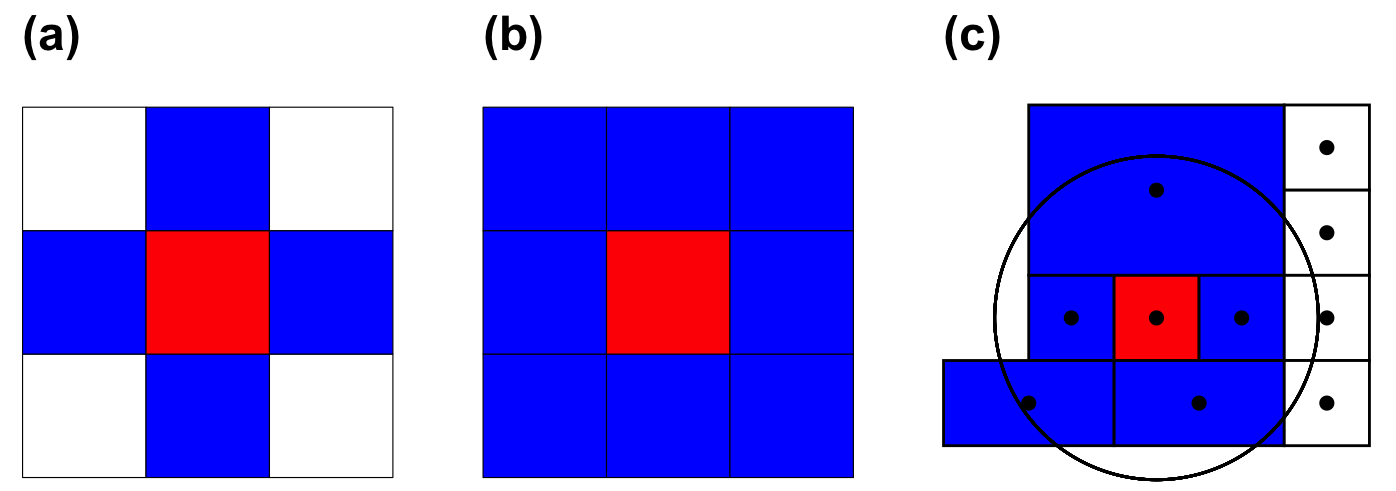
\includegraphics[width=1.0\textwidth]{figures/Neighbors/RookQueen2ndContiguityColored.png}
\caption{(a) Rook neighbors (blue) share an edge with a reference spatial region (red), (b) Queen neighbors (blue) share either an edge or vertex (or both) with a reference spatial region (red), and (c) Distance-based neighbors (blue) have centroids within a fixed radius of the reference cluster (red). Clusters with centroids beyond this distance are not considered as neighbors (white)\cite{moraga_spatial_2024}}
\label{figure:NeighborPlots}
\end{figure}

% \begin{figure} [!ht]
% \centering
% 
\includegraphics[width=0.60\textwidth]{figures/Neighbors/RookContiguity.png}
% \caption{Rook neighbors (light) share an edge with a reference spatial region (dark)\cite{moraga_spatial_2024}}
% \label{figure:RookContiguity}
% \end{figure}

% \begin{figure} [!ht]
% \centering
% 
\includegraphics[width=0.60\textwidth]{figures/Neighbors/QueenContiguity.png}
% \caption{Queen neighbors (light) share either an edge or vertex (or both with a reference spatial region (dark)\cite{moraga_spatial_2024}}
% \label{figure:QueenContiguity}
% \end{figure}

% Rook & Queen Neighbors
% \begin{figure}[!ht]
%     \centering % Center the entire figure environment
%     % First Figure (Rook Contiguity)
%     \begin{minipage}{0.48\textwidth} % Set width to slightly less than half of the text width
%         \centering % Center the image within its minipage
%         
\includegraphics[width=\linewidth]{figures/Neighbors/RookContiguityNoTitle.png} % Use \linewidth to fit image to minipage width
%         \caption{Rook neighbors (light) share an edge with a reference spatial region (dark)\cite{moraga_spatial_2024}}
%         \label{figure:RookContiguity}
%     \end{minipage}% <-- **THIS PERCENT SIGN IS CRUCIAL!**
%     \hfill % \hfill puts a flexible horizontal space between minipages
%     % Second Figure (Queen Contiguity)
%     \begin{minipage}{0.48\textwidth} % Set width to slightly less than half of the text width
%         \centering % Center the image within its minipage
%         
\includegraphics[width=\linewidth]{figures/Neighbors/QueenContiguityNoTitle.png} % Use \linewidth to fit image to minipage width
%         \caption{Queen neighbors (light) share either an edge or vertex (or both) with a reference spatial region (dark)\cite{moraga_spatial_2024}}
%         \label{figure:QueenContiguity}
%     \end{minipage}

%     % Changed to a regular \caption for a numbered figure, which is more common.
%     % If you specifically want an unnumbered caption, revert to \caption*{...}.
%     %\caption{Comparison of Rook and Queen Contiguity Definitions}
%     %\label{figure:ContiguityComparison} % Overall label for the combined figure
% \end{figure}

% $\textbf{Bishop}$ Neighbors that share a common boundary at the vertex (corners) of the spatial region are known as Bishop neighbors\cite{fotheringham_sage_2009}.

% $\textbf{Higher-Order Neighbors}$ Spatial regions that do not directly share an edge and/or vertex with another region, but instead share an edge and/or vertex with neighbors of a region are higher-order neighbors. Figure~\ref{figure:HigherOrderNeighbors} illustrates a comparison between the first order neighbors for rook and queen contiguity (top row) versus the second order neighbors for rook and queen contiguity. These higher-order neighbors are ``neighbors of neighbors" of the reference cell.

% \begin{figure} [!ht]
% \centering
% 
\includegraphics[width=0.70\textwidth]{figures/Neighbors/HigherOrderNeighbors.png}
% \caption{Higher order neighbors (light) are ``neighbors of neighbors" of a reference cell (darkest)\cite{moraga_spatial_2024}. Rook neighbors (left) share edge boundaries and Queen neighbors (right) share either edge or vertex boundaries.}
% \label{figure:HigherOrderNeighbors}
% \end{figure}

\subsubsection{Distance-Based}

Distance-based neighbors\cite{fotheringham_sage_2009} are constructed with the assumption that neighbors of a given area (individual cells in the case of this study) are other areas (or cells) that lie within a specified distance of another cell or observation. This distance is commonly defined by the radius of a circle around the center of a reference spatial region. The region specified in Figure~\ref{figure:NeighborPlots} (c) identifies distance-based neighbors of the reference cell (dark) as neighboring cells where the centroid of the cells is within the circumscribed boundary around the reference cell. In addition to cells, distance-based neighborhoods can also be constructed based on individual points that are within a specified distance of another point.

% \begin{figure} [!ht]
% \centering
% 
\includegraphics[width=0.60\textwidth]{figures/Neighbors/DistanceBasedNeighbors.png}
% \caption{Distance-based neighbors (light) have centroids within a fixed radius of the reference cluster (dark). Clusters with centroids beyond this distance are not considered as neighbors (white)\cite{moraga_spatial_2024}}
% \label{figure:DistanceBasedNeighbors}
% \end{figure}

\subsection{Intervention \& Spillover Effects}

Two primary effect types are considered to understand how treatments affect subjects in clusters where they are applied and subjects in the surrounding areas. The intervention effect and spillover effect are two parameters that are estimated in this study. Spatial cluster randomized trials have subjects or regions that are assigned to receive an intervention and others assigned as controls that do not receive an intervention. Observation of the resulting outcomes allows for estimation of the direct intervention effect and indirect spillover effect on the study region.

\subsubsection{Intervention Effect}\label{Section:InterventionEffect}

The intervention effect ($\beta$) represents the estimated effect of the direct intervention applied in a study. This is a measure of the study outcome that is directly attributed to the intervention applied in the study. Estimation of this intervention effect is possible due to the presence of clusters assigned as a control for comparison. The relevant intervention could be a vaccine to prevent infectious disease, a training program for government employees, an educational program for students, or many others. 

%%% INTERVENTION EFFECT EQUATION (SIMPLE MODEL) %%%
% The response $y$ for subject $i$ considering the intervention effect $\beta$ is expressed as
% \begin{equation}
%     y_i = \alpha + \beta x_i + \varepsilon_i
% \end{equation}
% where $x_i$ is an indicator of whether subject $i$ receives the intervention, $\alpha$ is a baseline effect, and $\varepsilon_i$ is a random error term for subject $i$.

\subsubsection{Spillover Effect Methods}\label{Section:SpilloverEffectMethods}

The spillover effect ($\psi$) represents an indirect effect on clusters where an intervention was not directly applied\cite{benjamin-chung_spillover_2017}\cite{benjamin-chung_extension_2024}. There are many to model a spillover effect as it is observed due to spatial proximity to subjects or regions where an intervention is applied. In this study, only binary spillover effects were considered. A binary spillover effect is a fixed level of a spillover effect that is applied if a subject or region is deemed to be a neighbor of a subject or region where the intervention is applied. 

%%% SPILLOVER EFFECT EQUATION (SIMPLE MODEL) %%%
% The response for subject $i$ considering this spillover effect is expressed as
% \begin{equation}
%     y_i = \alpha + \beta x_i +\psi z_i + \varepsilon_i.
% \end{equation}
% where $z_i$ is an indicator of whether the same subject neighbors another subject that receives the intervention and is eligible to experience spillover, $\psi$ is the maximum proportion of the intervention effect that can be experienced as spillover - in this case the binary effect applies 100\% of possible spillover, and $\alpha$, $\beta$, $x_i$, \& $\varepsilon_i$ are as described in Section~\ref{Section:InterventionEffect}. Alternative methods of modeling a spillover effect include: linear, categorical, exponential, and other decay functions\cite{jarvis_spatial_2018}\cite{bian_dual_2025}.

% but some alternative spillover methods are also discussed. In the following definitions, $x_i$ is an indicator of whether subject $i$ receives the intervention, $z_i$ is an indicator of whether the same subject neighbors another subject that receives the intervention (1) or not (0) and is eligible to experience spillover, $d_{\text{max}}$ is the diameter of each cluster of uniform size, $d_i$ is the distance that a subject is from the nearest intervention source, and $\psi$ is the maximum proportion of the intervention effect that can be experienced as spillover.

% \begin{itemize}
%     \item $\textbf{Binary}$: a fixed level of a spillover effect is applied if a subject or region is deemed to be a neighbor of a subject or region where the intervention is applied. This response for subject $i$ considering this spillover effect is expressed as
%     \begin{equation*}
%         y_i = \alpha + \beta x_i +\psi z_i + \varepsilon_i.
%     \end{equation*}
    
%     \item $\textbf{Linear}$: The effect of an intervention can decay as distance from the treatment sources increases. A linear decay spillover effect can be applied such that subjects closer to others receiving an intervention experience a greater spillover effect (larger proportion of the intervention effect) and those a greater distance from an intervention source receive a lesser effect (or none) from the intervention. The response for a subject $i$ with a linear decay spillover effect is
%     \begin{equation*}
%         y_i = \alpha + \beta x_i + \psi\left(1 - \frac{d_i}{d_{\text{max}}}\right)z_i
%     \end{equation*}

%     \item $\textbf{Categorical}$: A categorical decay spillover effect models a step-wise drop-off in the proportion of the intervention effect experienced at increasing levels of distance from the nearest intervention source. Contrary to the linear spillover effect, a categorical spillover effect allows for a constant effect to be experienced at concentric bands of distance from an intervention source. Subject $i$ has the following response with consideration of a categorical spillover effect
%     \begin{align*}
%         y_i &= \alpha + \beta x_i + \psi\biggl[I\left(d_i \in \left[0, \frac{1}{4}d_{\text{max}}\right]\right)
%         + 0.75 I\left(d_i \in \left[\frac{1}{4}d_{\text{max}}, \frac{1}{2}d_{\text{max}}\right]\right)\\ &+ 0.50 I\left(d_i \in \left[\frac{1}{2}d_{\text{max}}, \frac{3}{4}d_{\text{max}}\right]\right)
%         + 0.25 I\left(d_i \in \left[\frac{3}{4}d_{\text{max}}, d_{\text{max}}\right]\right)\biggr]z_i,
%     \end{align*}
    
%     Here, each of the domains of $d_i$ denotes a ``concentric" ring of distance from the intervention zone that receives a certain proportion of the intervention effect (decays in step with distance from the intervention zone). The rings here are the first, second, third, and fourth quartiles of distance from an intervention boundary with respect to the diameter of a cluster.
    
%     \item $\textbf{Exponential}$: An exponential decay pattern of spillover has a much ``steeper" drop-off in the effect experienced by a subject neighboring an intervention cluster as the distance from the intervention source increases. This is a reasonable model for spillover if subjects nearby an intervention are expected to experience a strong spillover effect, but subjects that a marginally larger distance and beyond experience little to no effect in the form of spillover. The response for subject $i$ with an exponential decay spillover effect is
%     \begin{equation*}
%         y_i = \alpha + \beta x_i + \psi\biggl[\text{exp}\left(-k \frac{d_i}{d_{\text{max}}}\right)\biggr]z_i,
%     \end{equation*}

%     where $k$ denotes the decay rate of the exponential function.
    
%     \item $\textbf{Gaussian}$: A Gaussian decay spillover appears as a ``bell"-shaped distribution when the effect strength is plotted against distance. This decay pattern is similar to exponential decay, but the effect decay is much slower at first before a steep drop-off in effect strength occurs at a moderate to large distance from the intervention source. The response for subject $i$ with a gaussian decay spillover effect (and spread parameter $\sigma$) is
%     \begin{equation*}
%         y_i = \alpha + \beta x_i + \psi\text{exp}\left(-\frac{d_{i}^{2}}{2\sigma^2}\right)z_i,
%     \end{equation*}

%     where small $\sigma$ correspond to a rapid decay of the spillover effect and large $\sigma$ allow for a much larger distance of spillover effect decay.
% \end{itemize}

\subsubsection{Spillover Effect Types}\label{section:SpilloverEffectTypes}

In this study, there are two specific ways in which spillover of the applied intervention is allowed to propagate to other cells or subjects. In both cases, spillover effects originate from areas where the original intervention treatment is applied. The first case allows for spillover to propagate from cells receiving the intervention into only cells assigned as control cells. In this case, the effect of the intervention is not permitted to spillover into other intervention cells. This suggests a case where the intervention effect applied is the maximum observable effect and any potential spillover cannot increase the observed effect of a particular intervention. Another method of spillover application is considered where spillover effects are permitted to be applied to both control AND intervention cells that are neighbors of a cell that receives an intervention. This application suggests that an effect greater than that of the original intervention applied can potentially be observed in a cell that received an intervention and also had spillover from another intervention cell. It is also to be expected that any change in the estimated effects would not be observed in spatial settings where the treatment allocation does not satisfy block stratification conditions (where no intervention cells are rook neighbors with other intervention cells). Figure~\ref{figure:TrtNoSpillVsTrtSpill} provides a comparative representation of how these two methods permit the application of spillover effects on clusters based on their treatment assignment. In all scenarios of this simulation study, the application of any spillover effect is simply a binary indication of whether a cluster receives a spillover effect or not. Even if spillover exposure could potentially be directed from multiple neighboring clusters, the modeling in this study does not consider any additive spillover effects.

\begin{figure} [!ht]
\centering
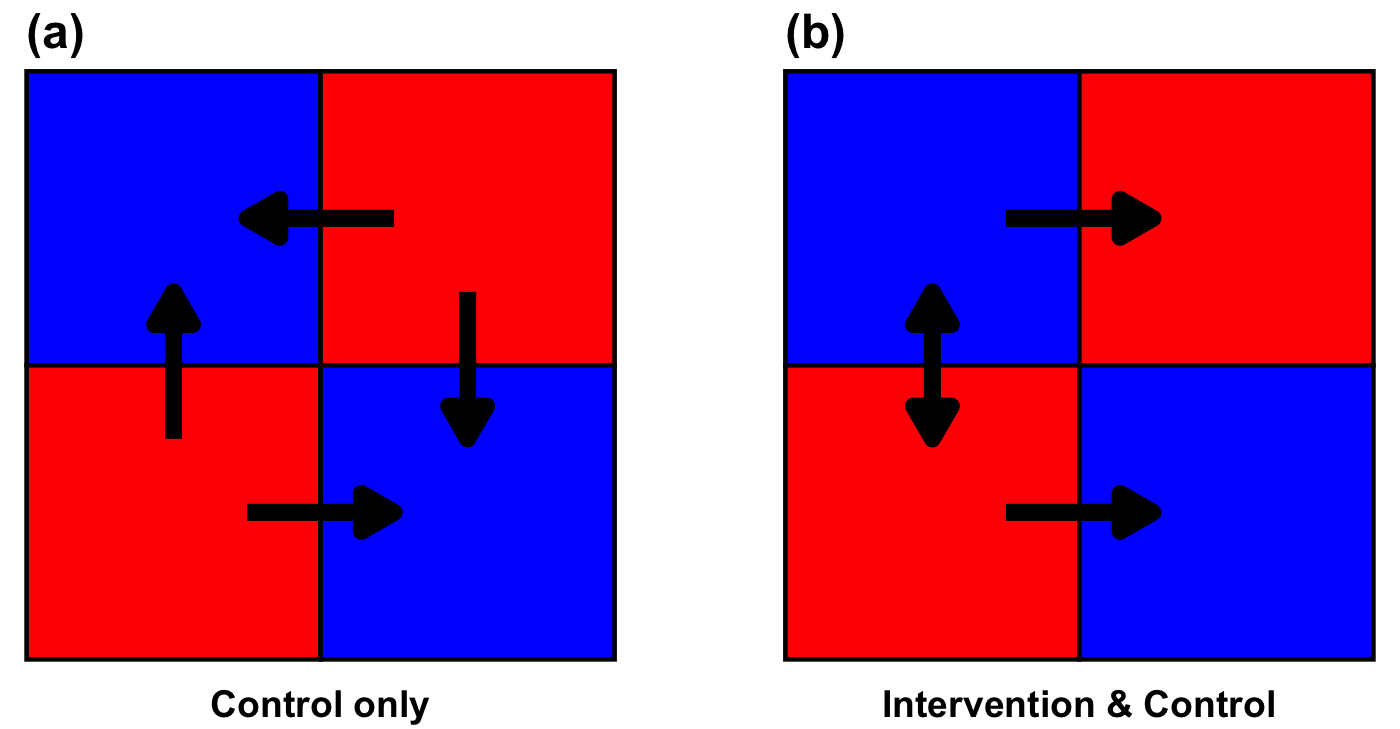
\includegraphics[width=0.80\textwidth]{figures/InterventionSpilloverEffect/TrtSpillComparisonV2.png}
\caption{(a) Spillover application from intervention cells (red) to only control cells (blue) \& (b) spillover application to intervention (red) and control cells (blue).}
\label{figure:TrtNoSpillVsTrtSpill}
\end{figure}

\subsection{Simple Random vs. Block Stratified Sampling}

In this study, two different treatments are considered: intervention $\&$ control. Assignment of these treatments is considered under two sampling methods: Simple Random Sampling (SRS) $\&$ Block Stratified Sampling (BSS). Random sampling treatment assignment considers all possible combinations of intervention $\&$ control arrangements on a specified spatial grid and provides equal probability of assignment for any given combination of intervention and control. For example, a 2 row by 3 column spatial grid has 6 total cells. Consideration of a 1:1 ratio between intervention and control treatments provides that three cells are assigned as intervention and three cells are assigned as control. Therefore, there are %$\binom{6}{3}=20$ 
$_{6}C_{3}=20$ different combinations of treatments for this specific spatial region. 

Block stratified sampling ensures a balanced number of intervention and control cells are selected, with the added condition that no intervention or control cells share a common edge boundary. An exception to this rule occurs in spatial setups where both dimensions are odd. In this case, the count of intervention and control cells must be out of balance and we assert that the control class will always be in the majority. In these instances, we relax the common edge boundary restriction for control cells and only require that intervention cells not share a common edge boundary in order to satisfy the block stratification condition.

We now consider a series of spatial grid setups to address efficient estimation of the intervention effect. These spatial grids are have dimensions denoted as (row $\times$ column) and we seek to apply a balanced distribution between intervention and control cells where possible. When this isn't possible, we defer to the control group being the majority class as mentioned previously.

\subsubsection{2x4 Grid}

One representative spatial setting considered is grid of 8 individual cells laid out in an arrangement of 2 rows and 4 columns. For this grid setup, a balanced set of intervention and control cells can be assigned where 4 cells are intervention regions and 4 cells are control regions. For a grid of 8 total cells and 4 cells of each treatment type, there are %$\binom{8}{4}=70$
$_{8}C_{4}=70$ unique arrangements of treatment and control assignments. Figure~\ref{figure:GridsCombined} (a) displays one of these combinations that satisfies the block stratified condition where intervention and control cells do not have any rook neighbors of the same treatment type. For this spatial setting, there are 2 (out of 70) combinations that satisfy the block stratification condition. Figure~\ref{figure:GridsCombined} (b) displays an example of the 2x4 grid spatial setting with a randomly sampled arrangement of intervention and control cells. Note that both treatment types have cells that are rook neighbors with the same treatment. These spatial grids are constructed with Simple Features for R package\cite{pebesma_simple_2018}\cite{pebesma_spatial_2023}.

% Figure: Combined Grids (2x4, 3x3, 3x4)
\begin{figure} [!ht]
\centering
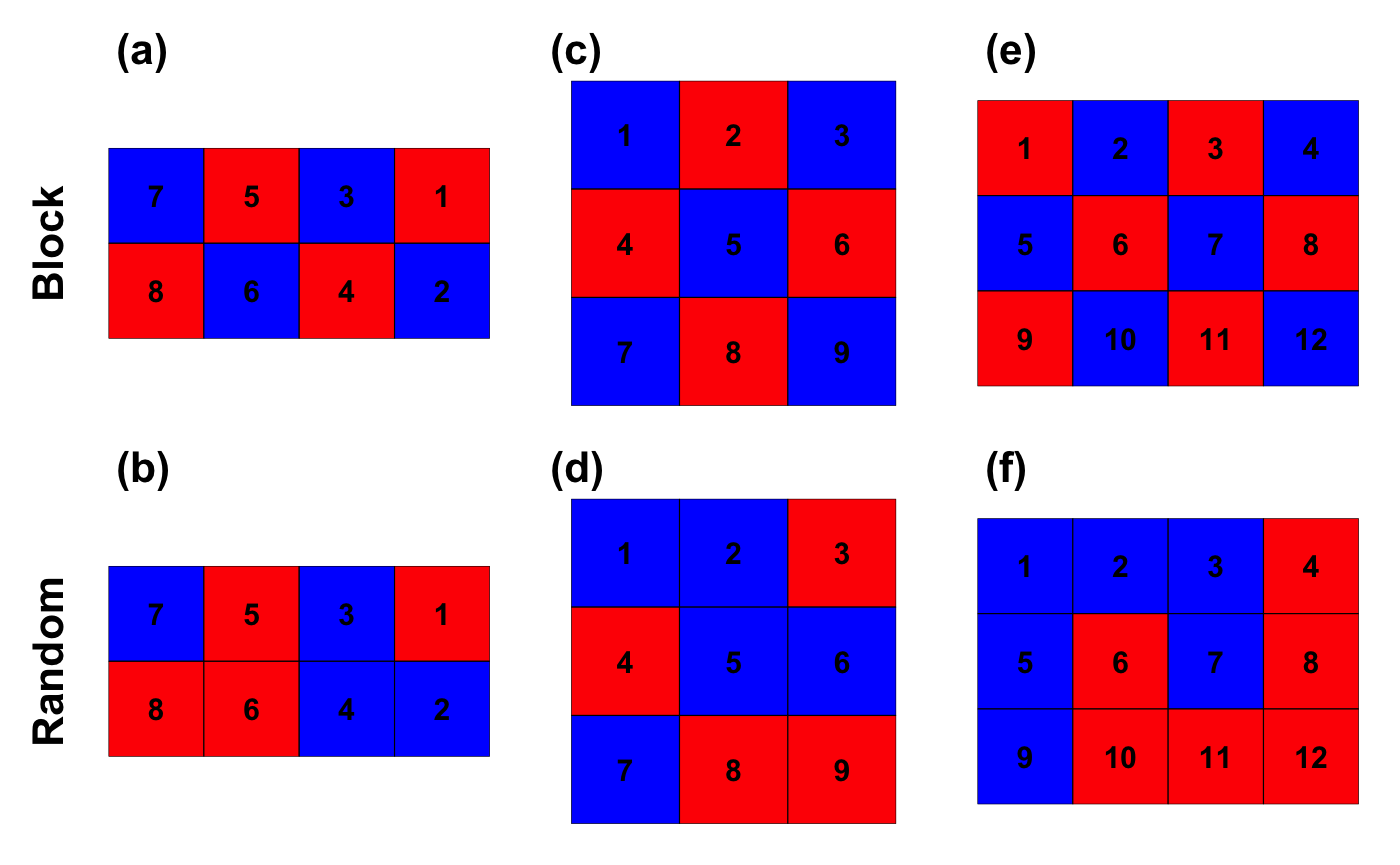
\includegraphics[width=1.0\textwidth]{figures/SpatialGridSetups/GridsCombined.png}
\caption{2x4 (left), 3x3 (middle), and 3x4 (right) spatial grids of intervention (red) and control (blue) clusters assigned via Block Stratified Sampling (top row) and Random Sampling (bottom row)}
\label{figure:GridsCombined}
\end{figure}

% 2x4 Block & Random Grids
% \begin{figure}[!ht]
%     \centering % Centers the entire block of minipages

%     % Left Column Figure
%     \begin{minipage}{0.45\textwidth} % Minipage for the left figure
%         \centering % Centers image within its minipage
%         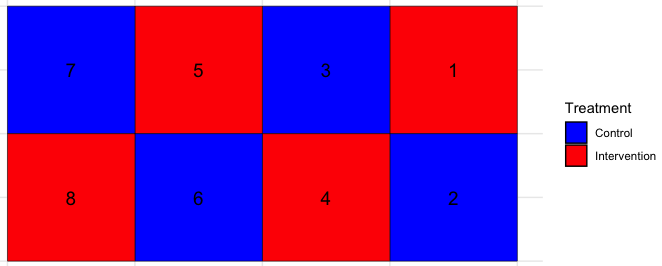
\includegraphics[width=\linewidth]{figures/SpatialGridSetups/Block/BlockStratificationSetup.png}
%         \caption{2x4 spatial grid of intervention (red) and control (blue) clusters assigned via Block Stratified Sampling}
%         \label{figure:BlockStratificationSetup}
%     \end{minipage}%\hspace*{\fill}%  <--- CRITICAL: Ensure NO actual newline character, blank line, or extra spaces between this '%' and the '\begin{minipage}' below. This entire sequence should be one continuous "line" in your .tex file.
%     \hfill % \hfill puts a flexible horizontal space between minipages
%     \begin{minipage}{0.45\textwidth} % Minipage for the right figure
%         \centering % Centers image within its minipage
%         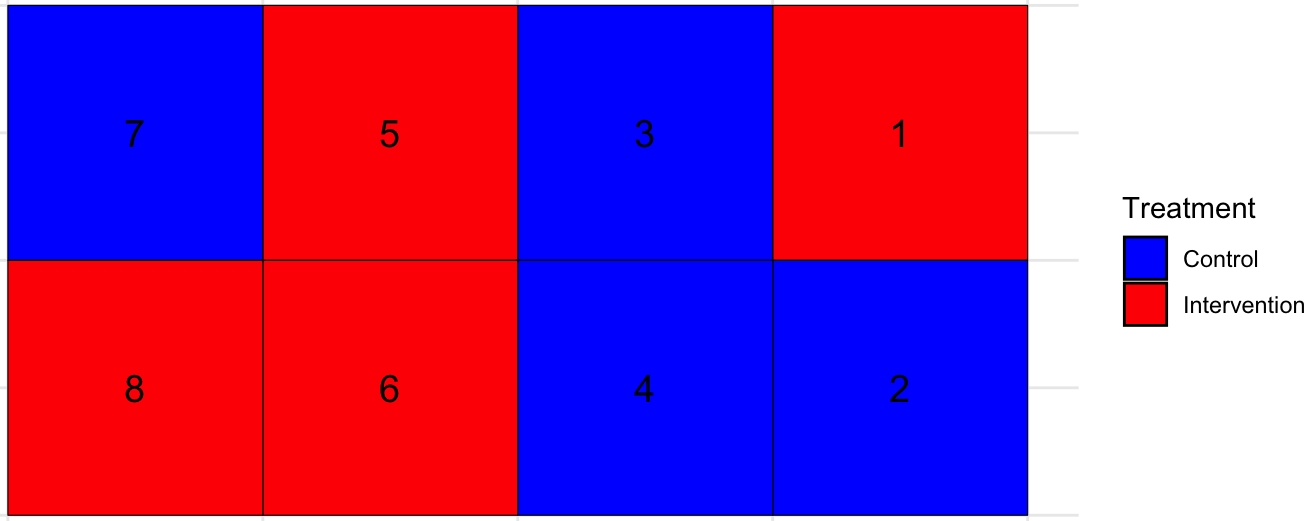
\includegraphics[width=\linewidth]{figures/SpatialGridSetups/Random/RandomSamplingExample2x4.png}
%         \caption{2x4 spatial grid of intervention (red) and control (blue) clusters assigned via Simple Random Sampling}
%         \label{figure:RandomSamplingExample2x4}
%     \end{minipage}

%     % Overall figure caption
%     %\caption{Comparison of intervention (red) and control (blue) clusters assigned via Block Stratified Sampling (left) and Simple Random Sampling (right) on a 2x4 Grid}
%     %\label{figure:SamplingComparison2x4}
% \end{figure}

%%%%%%%%%%%%%%%%%%%%

% \begin{figure} [!ht]
% \centering
% 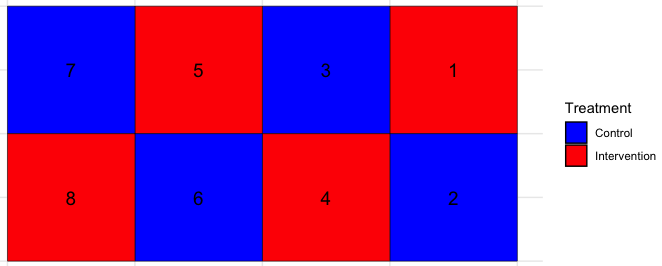
\includegraphics[width=0.70\textwidth]{figures/SpatialGridSetups/Block/BlockStratificationSetup.png}
% \caption{2x4 spatial grid of intervention (red) and control (blue) clusters assigned via Block Stratified Sampling}
% \label{figure:BlockStratificationSetup}
% \end{figure}

% \begin{figure} [!ht]
% \centering
% 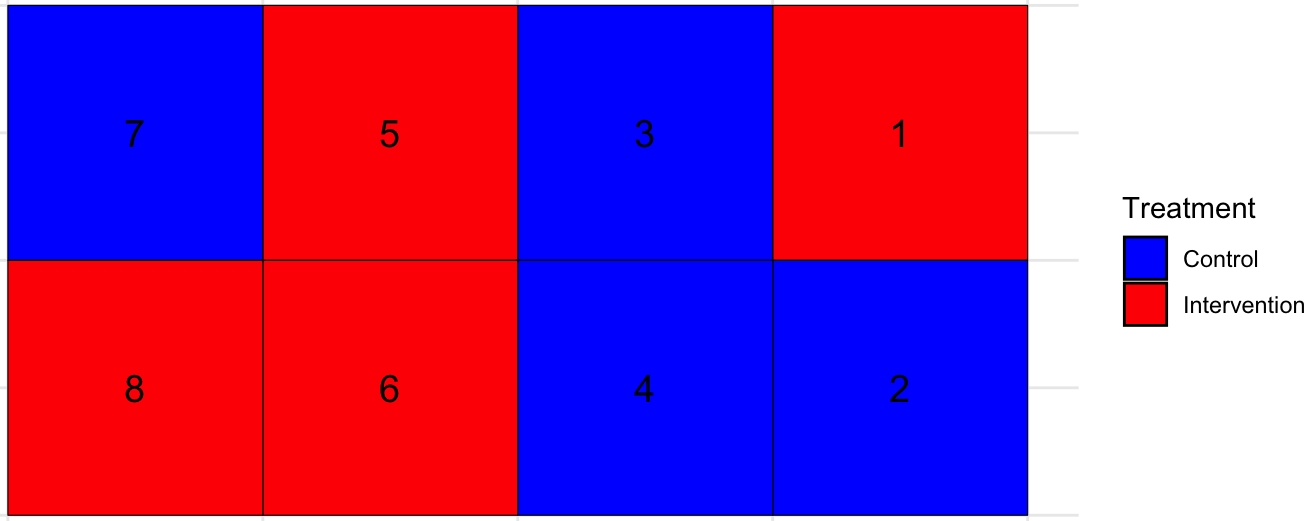
\includegraphics[width=0.70\textwidth]{figures/SpatialGridSetups/Random/RandomSamplingExample2x4.png}
% \caption{2x4 spatial grid of intervention (red) and control (blue) clusters assigned via Simple Random Sampling}
% \label{figure:RandomSamplingExample2x4}
% \end{figure}

\subsubsection{3x3 Grid}

The 3x3 symmetric grid setting of 9 cells allows for %$\binom{9}{4}=\binom{9}{5}=126$ 
$_{9}C_{4}=_{9}C_{5}=126$ unique combinations of intervention and control cells where 5 cells are allocated as control and 4 cells are treatment regions. The majority class of 5 cells is the control group for the sake of hypothetical resource management. Figure~\ref{figure:GridsCombined} (c) illustrates one combination of treatment and control cells that completely satisfies the block stratification conditions. Additional cluster combinations satisfy a relaxed condition of block stratification where control cells are allowed to have other control cells as rook neighbors. This is possible in spatial grid settings where both dimensions (row, column) are odd in length. There is one combination for the 3x3 grid setting that satisfies the strongest block stratification condition and 5 more combinations that satisfy the relaxed block stratification condition for a total of 6. An example of random sampling treatment assignment that doesn't satisfy block stratification conditions is provided in Figure~\ref{figure:GridsCombined} (d).

% 3x3 Block & Random Grids
% \begin{figure}[!ht]
%     \centering % Centers the entire block of minipages

%     % Left Column Figure
%     \begin{minipage}{0.45\textwidth} % Minipage for the left figure
%         \centering % Centers image within its minipage
%         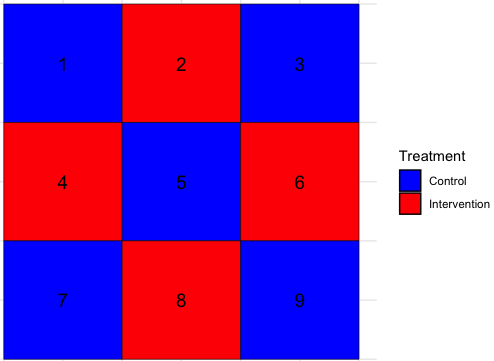
\includegraphics[width=\linewidth]{figures/SpatialGridSetups/Block/BlockStratification3x3.png}
%         \caption{3x3 spatial grid of clusters with intervention (red) and control (blue) assigned via Block Stratified Sampling}
%         \label{figure:BlockStratification3x3}
%     \end{minipage}%\hspace*{\fill}%  <--- CRITICAL: Ensure NO actual newline character, blank line, or extra spaces between this '%' and the '\begin{minipage}' below. This entire sequence should be one continuous "line" in your .tex file.
%     \hfill % \hfill puts a flexible horizontal space between minipages
%     \begin{minipage}{0.45\textwidth} % Minipage for the right figure
%         \centering % Centers image within its minipage
%         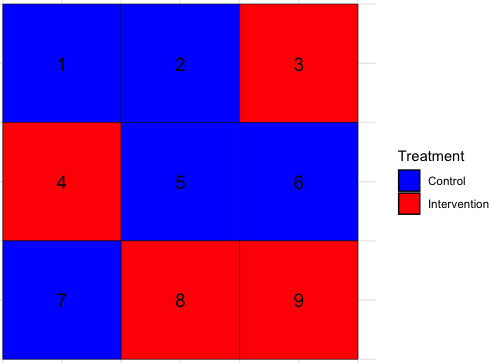
\includegraphics[width=\linewidth]{figures/SpatialGridSetups/Random/RandomSamplingExample3x3.png}
%         \caption{3x3 spatial grid of intervention (red) and control (blue) clusters assigned via Simple Random Sampling}
%         \label{figure:RandomSamplingExample3x3}
%     \end{minipage}

%     % Overall figure caption
%     % \caption{Comparison of intervention (red) and control (blue) clusters assigned via Block Stratified Sampling (left) and Simple Random Sampling (right) on a 3x3 Grid}
%     % \label{figure:SamplingComparison3x3}
% \end{figure}

%%%%%%%%%%%%%%%%%%%%

% 3x3 Individual Grids
% \begin{figure} [!ht]
% \centering
% 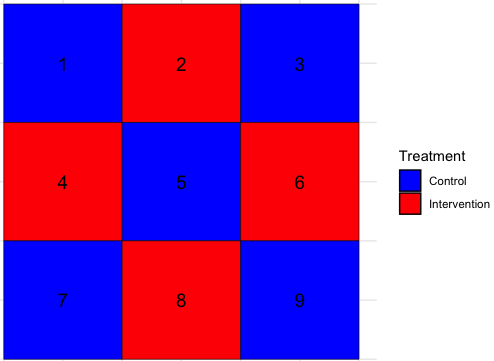
\includegraphics[width=0.70\textwidth]{figures/SpatialGridSetups/Block/BlockStratification3x3.png}
% \caption{3x3 spatial grid of clusters with intervention (red) and control (blue) assigned via Block Stratified Sampling}
% \label{figure:BlockStratification3x3}
% \end{figure}

% \begin{figure} [!ht]
% \centering
% 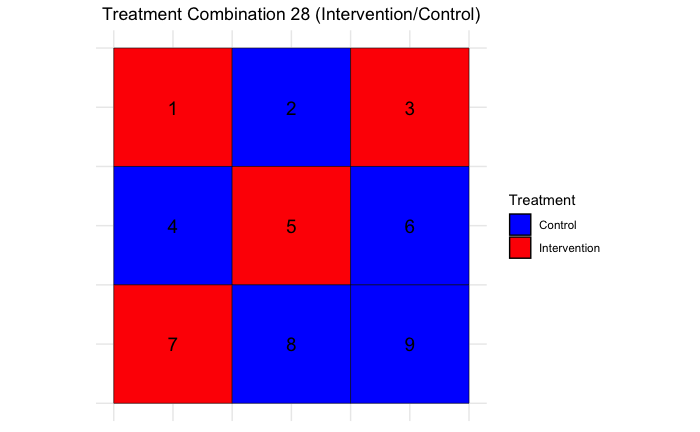
\includegraphics[width=0.70\textwidth]{figures/SpatialGridSetups/Block/BlockStratificationIntSep3x3.png}
% \caption{3x3 spatial grid of intervention (red) and control (blue) clusters assigned via relaxed Block Stratified Sampling}
% \label{figure:BlockStratificationIntSep3x3}
% \end{figure}

% \begin{figure} [!ht]
% \centering
% 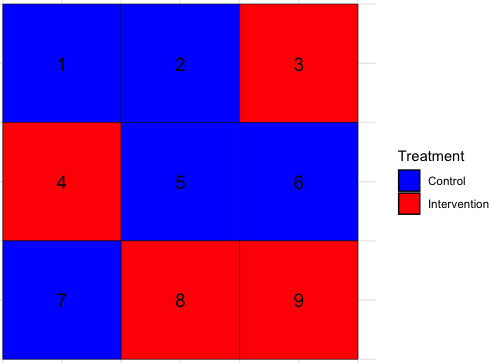
\includegraphics[width=0.70\textwidth]{figures/SpatialGridSetups/Random/RandomSamplingExample3x3.png}
% \caption{3x3 spatial grid of intervention (red) and control (blue) clusters assigned via Simple Random Sampling}
% \label{figure:RandomSamplingExample3x3}
% \end{figure}

\subsubsection{3x4 Grid}

The final spatial setting considered was a 3 row by 4 column (3x4) grid of 12 total cells. This grid, with a balanced allocation of 6 intervention cells and 6 control cells allows for %$\binom{12}{6}=924$
$_{12}C_{6}=924$ unique arrangements of the two treatments in the spatial region. For this particular grid size, 2 of the 924 treatment combinations satisfy the block stratification condition and Figure~\ref{figure:GridsCombined} (e) presents one of these, with a ``checkerboard" design. The remaining treatment combinations are achieved via random sampling of a balanced number of intervention and control cells. Figure~\ref{figure:GridsCombined} (f) illustrates another randomly sampled arrangement of the treatments onto the spatial area where control and intervention cells each have rook neighbors of the same treatment type.

% 3x4: Block & Random Grids
% \begin{figure}[!ht]
%     \centering % Centers the entire block of minipages

%     % Left Column Figure
%     \begin{minipage}{0.45\textwidth} % Minipage for the left figure
%         \centering % Centers image within its minipage
%         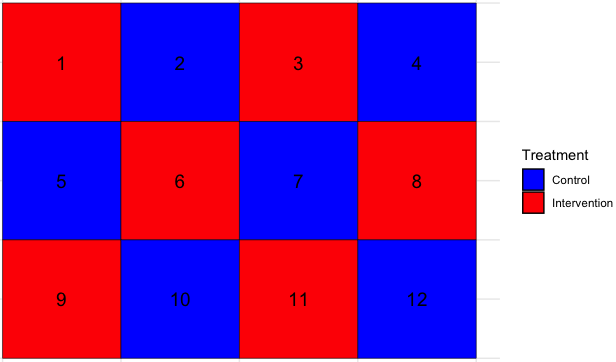
\includegraphics[width=\linewidth]{figures/SpatialGridSetups/Block/BlockStratification3x4.png}
%         \caption{3x4 spatial grid of clusters with intervention (red) and control (blue) assigned via Block Stratified Sampling}
%         \label{figure:BlockStratification3x4}
%     \end{minipage}%\hspace*{\fill}%  <--- CRITICAL: Ensure NO actual newline character, blank line, or extra spaces between this '%' and the '\begin{minipage}' below. This entire sequence should be one continuous "line" in your .tex file.
%     \hfill % \hfill puts a flexible horizontal space between minipages
%     \begin{minipage}{0.45\textwidth} % Minipage for the right figure
%         \centering % Centers image within its minipage
%         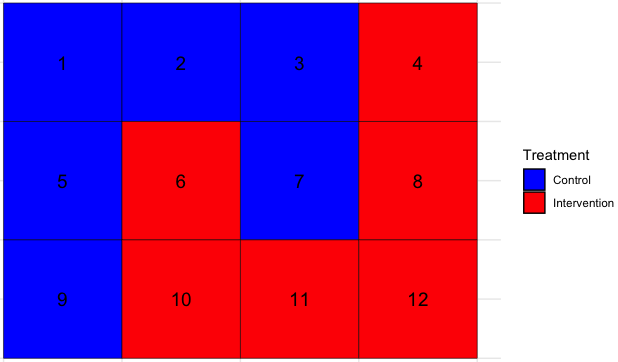
\includegraphics[width=\linewidth]{figures/SpatialGridSetups/Random/RandomSamplingExample3x4.png}
%         \caption{3x4 spatial grid of intervention (red) and control (blue) clusters assigned via Simple Random Sampling}
%         \label{figure:RandomSamplingExample3x4}
%     \end{minipage}

%     % Overall figure caption
%     % \caption{Comparison of intervention (red) and control (blue) clusters assigned via Block Stratified Sampling (left) and Simple Random Sampling (right) on a 3x4 Grid}
%     % \label{figure:SamplingComparison3x4}
% \end{figure}

%%%%%%%%%%%%%%%%%%%%

% 3x4: Individual Grids
% \begin{figure} [!ht]
% \centering
% 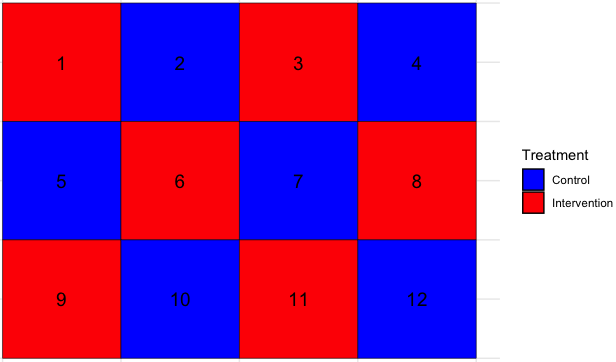
\includegraphics[width=0.70\textwidth]{figures/SpatialGridSetups/Block/BlockStratification3x4.png}
% \caption{3x4 spatial grid of clusters with intervention (red) and control (blue) assigned via Block Stratified Sampling}
% \label{figure:BlockStratification3x4}
% \end{figure}

% \begin{figure} [!ht]
% \centering
% 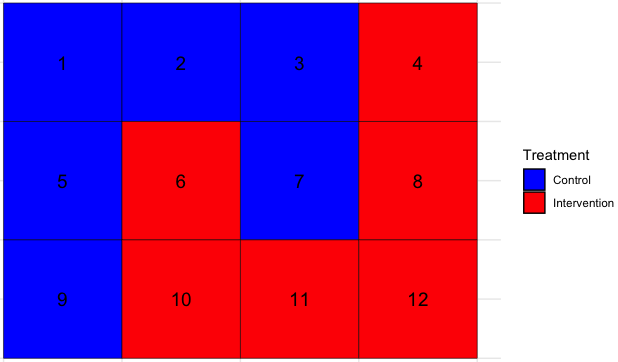
\includegraphics[width=0.70\textwidth]{figures/SpatialGridSetups/Random/RandomSamplingExample3x4.png}
% \caption{3x4 spatial grid of intervention (red) and control (blue) clusters assigned via Simple Random Sampling}
% \label{figure:RandomSamplingExample3x4}
% \end{figure}

\subsection{Spatial Autoregressive (SAR) Model}\label{section:SAR}

Outcomes in the presence of spatial dependence and spillover effects can be considered via modeling with a spatial autoregressive\\ model\cite{waller_applied_2004}\cite{fotheringham_sage_2009}\cite{ullah_handbook_1998}. A spatial autoregressive model has the form:

\begin{equation}\label{Equation:SARmodel}
    y_{ik} = \rho\sum_j w_{ij}y_{jk'} + \mathbf{x}_i \beta + \varepsilon_i
\end{equation}

\noindent where $k$ and $k'$ are different cluster indices for each individual, $\rho$ is the spatial correlation (autoregressive) coefficient, and $\varepsilon_i$ represents an i.i.d. error term. This can also be expressed in matrix notation as:

\begin{equation}
    \mathbf{y} = \rho\mathbf{Wy}+\mathbf{X}\beta + \varepsilon
\end{equation}
It follows that the general form of the response for this model for the purpose of this study is
\begin{equation}
    y_{ik} = \alpha + \beta x_{ik} + \psi z_{ik} + \rho\mathbf{Wy} + \epsilon_i
\end{equation}
where $y_i$ is the observed response for subject $i$, $\alpha$ is the baseline effect, $\beta$ is the intervention effect, $x_i$ is an indicator of whether subject $i$ receives the intervention, $\psi(d_i)$ is the spillover effect expressed as a function of distance from the nearest intervention source for subject $i$, $z_i$ is an indicator of whether subject $i$ can experience any spillover effect, and $\rho\mathbf{Wy}$ captures spatial dependence from neighboring observations and their effects in the response variable. The components of $\rho\mathbf{Wy}$ are $\rho$, a fixed spatial correlation parameter, $\mathbf{W}$, the spatial weights matrix indicating the strength of relationship between neighboring observations, and the response vector $\mathbf{y}$. Finally, $\varepsilon_i$ is a random error term for each subject.

\subsection{Spatial Dependence}\label{section:SpatialWeightsMatrix}

Spatial dependence, used interchangeably with spatial autocorrelation, refers to the property of spatial data where observations close to each other tend not be independent of each other. Rather, observations that are close to each other tend to be dependent on each other and influence values of surrounding data. Hence, there is an implied systematic correlation between data at neighboring locations. Spatial correlation can be positive, where similar values tend to be clustered close together, or negative, where dissimilar values are close together. Appropriate consideration of spatial dependence is necessary for performing valid statistical inference as well as for accurate estimation of effects that are modeled. A pair of common methods for assessing spatial autocorrelation are Moran's $\textit{I}$ \cite{moran_interpretation_1948}\cite{moran_notes_1950} and Geary's $\textit{C}$ \cite{geary_contiguity_1954}\cite{waller_applied_2004}. Moran's $\textit{I}$ standardizes the spatial auto-covariance by the variance of the data and Geary's $\textit{C}$ utilizes the sum of the squared differences between pairs of data as a measure of co-variation. These test statistics are reliant on the spatial weights matrix.

% \subsubsection{Tests of Spatial Dependence - Moran's \textit{I}}

% The Moran's $\textit{I}$ statistic quantifies the degree of similarity or dissimilarity between neighboring data using standardized spatial covariance. The statistic takes on values from -1 (negative autocorrelation) to 1 (positive autocorrelation) where the expected value under a null hypothesis of no spatial autocorrelation is $E\left[\textit{I}\right] = -\left(N-1\right)^{-1}$ , where $N$ is the count of spatial units. Moran's $\textit{I}$ has the form
% \begin{equation*}
%     \textit{I} = \frac{N\sum_{i=1}^{N}\sum_{j=1}^{N}w_{ij}\left(x_i - \bar{x}\right)\left(x_j-\bar{x}\right)}{\left(\sum_{i=1}^{N}\sum_{j=1}^{N}w_{ij}\right)\sum_{i=1}^{N}\left(x_i - \bar{x}\right)^2}
% \end{equation*}
% where
% \begin{itemize}
%     \item $N$ is the number of spatial units
%     \item $x_i$ is the value of a unit at location $i$
%     \item $\bar{X}$ is the average of the unit values
%     \item $w_{ij}$ are elements of the spatial weights matrix.
% \end{itemize}

% Moran's $\textit{I}$ can be implemented with the `moran.test()' function from the spdep package in R\cite{bivand_comparing_2018}.

% \subsubsection{Tests of Spatial Dependence - Geary's \textit{C}}

% The Geary's $\textit{C}$ statistic considers the sum of squared differences between adjacent observations or values. Values that are significantly less than 1 are an indication of rising positive spatial autocorrelation and values much higher than 1 represent increasing negative spatial correlation. Under the null hypothesis of no spatial autocorrelation, the expected value is $E\left[\textit{C}\right] = 1$. The applicable formula of the statistic is
% \begin{equation*}
%     \textit{C} = \frac{\left(N-1\right)\sum_{i=1}^{N}\sum_{j=1}^{N} w_{ij}\left(x_i-x_j\right)^2}{2\left(\sum_{i=1}^{N}\sum_{j=1}^{N}w_{ij}\right)\sum_{i=1}^{N}\left(x_i-\bar{x}\right)^2}
% \end{equation*}
% where
% \begin{itemize}
%     \item $N$ is the number of spatial units
%     \item $x_i$ and $x_j$ are unit values at locations $i$ and $j$
%     \item $\bar{x}$ is the average of the unit values
%     \item $w_{ij}$ are the elements of the spatial weights matrix.
% \end{itemize}

% Geary's $\textit{C}$ can be implemented with the `geary.test()' function from the spdep package in R\cite{bivand_comparing_2018}.

%\subsubsection{Spatial Weights Matrix}

The spatial weights matrix $\mathbf{W}$ is a component of the SAR model from Section~\ref{section:SAR}. It is composed elements $w_{ij}$ which indicate the strength or presence of a spatial connection between observations $i$ and $j$. Therefore the spatial dependence term of the SAR model is represented as

\begin{equation}
    \rho\mathbf{Wy} = \rho\sum_{j \in \mathcal{N}(i)}w_{ij}y_j
\end{equation}

where $\rho$ is the spatial autocorrelation parameter; an indicator of how strongly neighboring values affect the focal observation, $\mathbf{W}$ is the spatial weights matrix between subjects $i$ and $j$ with matrix elements $w_{ij}$ that are either indicator-based $(\{0,1\})$ or distance-based $\left(\frac{1}{d_{ij}}\right)$ where $d_{ij}$ is the distance between subjects $i$ and $j$, and $\mathcal{N}(i)$ is the set of all neighbors of observation $i$. In this study, this set consists of all subjects that are a member of a cluster that is a rook neighbor of the cluster of subject $i$. For the spatial weights matrix, The indicator-based weights are
\begin{equation}
    w_{ij} = 
    \begin{cases}
    1, \text{if points $i$ and $j$ are neighbors}\\
    0, \text{otherwise} 
    \end{cases}
\end{equation}
and are normalized via
\begin{equation}
    W_{ij} = \frac{w_{ij}}{\sum_{j}w_{ij}}
\end{equation}
and the distance-based weights are
\begin{equation}
    w_{ij} = 
    \begin{cases}
    \frac{1}{d_{ij}}, \text{if $0 < d_{ij} < d_{\text{max}}$}\\
    0, \text{otherwise} 
    \end{cases}
\end{equation}
which are normalized via
\begin{equation}
    W_{ij} = \frac{\frac{1}{d_{ij}}}{\sum_{j}\frac{1}{d_{ij}}}.
\end{equation}

\subsection{Estimation for SAR Model}

Maximum likelihood estimation is utilized to gather parameter estimates from the spatial lag \\ model from Section~\ref{section:SAR}\cite{ord_estimation_1975}\cite{bivand_comparing_2015}\cite{bivand_computing_2013}. When considering spatial dependence, the responses are

\begin{equation}
    y_i = \rho \sum_{j\neq i}w_{ij}y_{j} + \alpha + \beta x_i + \psi z_i + \epsilon_i
\end{equation}
where the residuals are
\begin{equation}
    \varepsilon_i = y_i - \rho \sum_{j\neq i}w_{ij}y_{j} - \left(\alpha + \beta x_i + \psi z_i\right).
\end{equation}

Then, assuming that $\varepsilon_i \sim N(0,\sigma^2)$, the likelihood function is

\begin{equation}
    L\left(\alpha, \beta, \psi, \rho, \sigma^2\right) = \frac{1}{\sqrt{\left(2\pi\sigma^2\right)^n |\mathbf{I}-\rho\mathbf{W}|}}\text{exp}\left(-\frac{1}{2\sigma^2}\epsilon^{\top}\epsilon\right)
\end{equation}
where $|\mathbf{I}-\rho\mathbf{W}|$ is the determinant of $\left(\mathbf{I}-\rho\mathbf{W}\right)$. The log-likelihood is
\begin{equation}
    \log L\left(\alpha, \beta, \psi, \rho, \sigma^2\right) = -\frac{n}{2}\log\left(2\pi\sigma^2\right)+\log|\mathbf{I}-\rho\mathbf{W}|-\frac{1}{2\sigma^2}\sum_{i=1}^{n}\left(y_i - \rho \sum_{j\neq i}w_{ij}y_{j} - \left(\alpha + \beta x_i +\psi z_i\right)\right)^2 
\end{equation}
which is maximized with respect to $\alpha, \beta, \psi, \rho, \text{ and } \sigma^2$. In applied simulation tasks, estimates can be obtained via the `lagsarlm()' function from the R spdep library\cite{bivand_r_2022}.

% --- SIMULATIONS (application) ---
\section{Simulation Study}

A simulation study was carried out to consider the contrast of block stratified and random treatment assignment sampling methods with consideration for spillover effects, spatial dependence, and restrictions on spillover application between intervention and control regions. The results of this study are detailed in the remainder of this section.

\subsection{Simulation Scenarios \& Response}

We carry out a simulation study to explore how estimation error of the intervention effect in a Spatial CRT varies across a range of spillover effect sizes, the presence or absence of spatial dependence, varying restrictions on clusters where spillover is permitted to occur, and the method of sampling for treatment assignment. Each simulation scenario is composed of a set of these parameters. The baseline effect, $\alpha$, is always assigned as $0.2$. The intervention effect, $\beta$, is always assigned as $1.0$. The spillover effect, $\psi$, has possible values $0.5$, $0.6$, $0.7$, and $0.8$. The spatial dependence parameter, $\rho$ is set as either $0.00$ or $0.01$. The sampling design for each scenario is either Block Stratified Sampling (BSS) or Simple Random Sampling (SRS). Finally, the spillover application type is (1) Control Clusters Only or (2) Control \& Intervention Clusters. Each simulation setting is replicated for each of the spatial grid dimensions discussed previously (2x4, 3x3, and 3x4).

Given that the form of the spatial lag model in Section~\ref{section:SAR} contains the response on both sides of the expression, a separate closed-form expression for data generation must be considered\cite{fotheringham_sage_2009}\cite{baltagi_spatial_2003}. This data generation expression is

\begin{equation}
    \mathbf{y} = \left(\mathbf{I}-\rho \mathbf{W}\right)^{-1}\left(\boldsymbol\alpha + \mathbf{X}\boldsymbol\beta + \epsilon\right)
\end{equation}
where $X\beta = \beta x_i + \psi z_i$. $x_i$ is an indicator of whether subject $i$ receives the intervention and $z_i$ is an indicator of whether subject $i$ receives any spillover effect.

% % --- REMOVE TABLE OF SCENARIOS
% \begin{table}[ht!]
% \centering
% \begin{tabular}{c c c c c c c}
%     \toprule
%     \textbf{Index} & \textbf{Alpha} & \textbf{Beta} & \textbf{\makecell{Spillover \\ Effect ($\psi$)}} & \textbf{\makecell{Spatial \\ Dependence ($\rho$)}} & \textbf{\makecell{Sampling \\ Design}} & \textbf{\makecell{Spillover Type}} \\
%     \midrule
%     % --- Control Only scenarios (Rows 1-16) ---
%     \textbf{Scenario 1} & 0.2 & 1.0 & 0.5 & 0.01 & SRS & Control Only \\
%     \textbf{Scenario 2} & 0.2 & 1.0 & 0.6 & 0.01 & SRS & Control Only \\
%     \textbf{Scenario 3} & 0.2 & 1.0 & 0.7 & 0.01 & SRS & Control Only \\
%     \textbf{Scenario 4} & 0.2 & 1.0 & 0.8 & 0.01 & SRS & Control Only \\
%     \cmidrule(lr){1-7}
%     \textbf{Scenario 5} & 0.2 & 1.0 & 0.5 & 0.00 & SRS & Control Only \\
%     \textbf{Scenario 6} & 0.2 & 1.0 & 0.6 & 0.00 & SRS & Control Only \\
%     \textbf{Scenario 7} & 0.2 & 1.0 & 0.7 & 0.00 & SRS & Control Only \\
%     \textbf{Scenario 8} & 0.2 & 1.0 & 0.8 & 0.00 & SRS & Control Only \\
%     \midrule
%     \textbf{Scenario 9} & 0.2 & 1.0 & 0.5 & 0.01 & BSS & Control Only \\
%     \textbf{Scenario 10} & 0.2 & 1.0 & 0.6 & 0.01 & BSS & Control Only \\
%     \textbf{Scenario 11} & 0.2 & 1.0 & 0.7 & 0.01 & BSS & Control Only \\
%     \textbf{Scenario 12} & 0.2 & 1.0 & 0.8 & 0.01 & BSS & Control Only \\
%     \cmidrule(lr){1-7}
%     \textbf{Scenario 13} & 0.2 & 1.0 & 0.5 & 0.00 & BSS & Control Only \\
%     \textbf{Scenario 14} & 0.2 & 1.0 & 0.6 & 0.00 & BSS & Control Only \\
%     \textbf{Scenario 15} & 0.2 & 1.0 & 0.7 & 0.00 & BSS & Control Only \\
%     \textbf{Scenario 16} & 0.2 & 1.0 & 0.8 & 0.00 & BSS & Control Only \\
%     \midrule
%     % --- Control & Intervention scenarios (Rows 17-32) ---
%     \textbf{Scenario 17} & 0.2 & 1.0 & 0.5 & 0.01 & SRS & Control \& Intervention \\
%     \textbf{Scenario 18} & 0.2 & 1.0 & 0.6 & 0.01 & SRS & Control \& Intervention \\
%     \textbf{Scenario 19} & 0.2 & 1.0 & 0.7 & 0.01 & SRS & Control \& Intervention \\
%     \textbf{Scenario 20} & 0.2 & 1.0 & 0.8 & 0.01 & SRS & Control \& Intervention \\
%     \cmidrule(lr){1-7}
%     \textbf{Scenario 21} & 0.2 & 1.0 & 0.5 & 0.00 & SRS & Control \& Intervention \\
%     \textbf{Scenario 22} & 0.2 & 1.0 & 0.6 & 0.00 & SRS & Control \& Intervention \\
%     \textbf{Scenario 23} & 0.2 & 1.0 & 0.7 & 0.00 & SRS & Control \& Intervention \\
%     \textbf{Scenario 24} & 0.2 & 1.0 & 0.8 & 0.00 & SRS & Control \& Intervention \\
%     \midrule
%     \textbf{Scenario 25} & 0.2 & 1.0 & 0.5 & 0.01 & BSS & Control \& Intervention \\
%     \textbf{Scenario 26} & 0.2 & 1.0 & 0.6 & 0.01 & BSS & Control \& Intervention \\
%     \textbf{Scenario 27} & 0.2 & 1.0 & 0.7 & 0.01 & BSS & Control \& Intervention \\
%     \textbf{Scenario 28} & 0.2 & 1.0 & 0.8 & 0.01 & BSS & Control \& Intervention \\
%     \cmidrule(lr){1-7}
%     \textbf{Scenario 29} & 0.2 & 1.0 & 0.5 & 0.00 & BSS & Control \& Intervention \\
%     \textbf{Scenario 30} & 0.2 & 1.0 & 0.6 & 0.00 & BSS & Control \& Intervention \\
%     \textbf{Scenario 31} & 0.2 & 1.0 & 0.7 & 0.00 & BSS & Control \& Intervention \\
%     \textbf{Scenario 32} & 0.2 & 1.0 & 0.8 & 0.00 & BSS & Control \& Intervention \\
%     \bottomrule
% \end{tabular}
% \caption{Simulation Scenarios for Intervention Estimation in 2x4, 3x3, and 3x4 Spatial Grid Setting}
% \label{table:SimulationSets}
% \end{table}

\subsection{Simulation Procedure}

The algorithm implemented to perform the simulations for this study is illustrated in the following section. The simulation is performed over all potential cluster treatment combinations (intervention/control) for each of the 2x4, 3x3, and 3x4 cluster spatial grid geometries. The simulation procedure is as follows:

\begin{enumerate}
    \item\label{DefineSpatialGeometry} Define the spatial grid geometry \& set of parameters for simulation scenario ($\alpha$, $\beta$, $\psi$, $\rho$)

    \item List out all cluster treatment combinations for specified spatial grid (70 combinations for 2x4, 126 combinations for 3x3, 924 combinations for 3x4

    \item Construct the spatial grid object for the corresponding number of clusters (8, 9, 12) and define the rook neighbors for each cluster in the spatial region.

    \item Identify cluster treatment combinations for the specified spatial grid object that satisfy Block Stratified Sampling (BSS) conditions (2x4: 2, 3x3: 6, 3x4: 2).

    \item\label{SimulationProcedure} For each combination in the set of all cluster treatment combinations for a given spatial grid:

    \begin{enumerate}
        \item Sample 20 subjects per cluster over the entire space of the grid (2x4: 160 subjects, 3x3: 180 subjects, 3x4: 240 subjects).

        \item Assign each subject to its corresponding cluster and to the intervention or control treatment based on the treatment assignment of the specific cluster.

        \item Identify the rook neighbors of each subject and whether each subject is exposed to a binary spillover effect based on the treatment assignment of neighboring clusters and selected spillover application type as described in Section~\ref{section:SpilloverEffectTypes}.

        \item Generate the response value for each subject with consideration for spatial dependence via Spatial Autoregressive (SAR) modeling.

        \item Estimate and retain parameter values for $\alpha, \beta, \psi, \text{ and } \rho$ with the Spatial simultaneous autoregressive lag model (`lagsarlm()`) via maximum likelihood estimation.

        \item Iterate parts (a)-(e) of Step~\ref{SimulationProcedure} N=50 times for each cluster treatment combination for the 2x4 and 3x3 spatial grids and N=10 times for each cluster treatment combination for the 3x4 spatial grid.
    \end{enumerate}

    \item Aggregate parameter estimates for each iteration of each cluster treatment combination for a specified spatial grid

    \item For each parameter estimate ($\alpha$, $\beta$, $\psi$, $\rho$), compute the bias of the mean of the estimates relative to the true value, variance of the estimates, and Mean Squared Error (MSE) of the estimates such that these metrics are computed for each cluster treatment combination.

    \item Repeat Steps~\ref{DefineSpatialGeometry}-\ref{SimulationProcedure} of the simulation procedure for each spatial grid setup (2x4, 3x3, 3x4).
\end{enumerate}

% % --- Refined Algorithm for Simulation Study --- (THIS NEEDS TO BE EDITED)
% \begin{algorithm}[ht!]
%     \caption{[EX: PLACEHOLDER] Simulation Algorithm for Intervention Effect ($\beta$) Estimation}
%     \label{alg:simulation_framework}
%     \begin{algorithmic}[1]
%         \Procedure{Simulate\_Spatial\_RCTs}{$\mathcal{S}, M$}
%         \Comment{$\mathcal{S}$: Set of all 32 simulation scenarios, $M$: Number of iterations per scenario}

%         \State \textbf{Construct Spatial Objects:}
%         \State Construct a spatial grid of $N=12$ clusters.
%         \State Define the spatial weights matrix $W$ based on cluster contiguity (e.g., Queen).
%         \State Define true parameters: $\beta=1.0$, and the ranges for $\psi$ and $\rho$.
%         \State Initialize a data structure to store final MSE and SD results for each scenario.

%         \For{each scenario $s$ in the set $\mathcal{S}$}
%             \Comment{Outer loop iterates through all 32 combinations}
%             \State Let $s = (\text{Sampling Design}, \rho, \psi, \text{Spillover Type})$.
%             \State Initialize an empty list $\mathcal{L}_{\hat{\beta}}$ to store estimates from this scenario.

%             \For{iteration $m=1, ..., M$}
%                 \Comment{Inner loop for Monte Carlo replicates}
%                 \State \textbf{Assign Treatment and Neighbors:}
%                 \State Assign $n_I=6$ intervention and $n_C=6$ control clusters based on the \textbf{Sampling Design}.
%                 \State Identify the set of neighbors for each cluster using the weights matrix $W$.
%                 \State Define spillover influence according to the \textbf{Spillover Type}.

%                 \State \textbf{Generate Data:}
%                 \State Generate outcome data $y$ for all clusters from a data generating process that includes:
%                 \Statex \qquad Spatial dependence (using parameter $\rho$),
%                 \Statex \qquad Intervention effect (using parameter $\beta$),
%                 \Statex \qquad Spillover effects (using parameter $\psi$).
%                 \Statex \qquad Example SAR model: $y = (I - \rho W)^{-1}(X\beta + Z\psi + \epsilon)$.

%                 \State \textbf{Fit Model and Estimate Parameters:}
%                 \State Fit a Spatial Autoregressive (SAR) model to the generated data.
%                 \State Estimate the intervention effect parameter $\hat{\beta}^{(m)}$ using Maximum Likelihood Estimation.
%                 \State Store the estimate: $\mathcal{L}_{\hat{\beta}} \gets \mathcal{L}_{\hat{\beta}} \cup \{\hat{\beta}^{(m)}\}$.

%             \EndFor \Comment{End of iteration loop}

%             \State \textbf{Aggregate Estimates for Scenario:}
%             \State Aggregate the stored estimates in $\mathcal{L}_{\hat{\beta}}$ across all $M$ iterations.
%             \State Compute the Mean Squared Error (MSE) and Standard Deviation (SD) for the estimated $\hat{\beta}$.
%             \State Record these aggregated metrics for scenario $s$.

%         \EndFor \Comment{End of scenario loop}

%         \State \Return Recorded MSE and SD for all scenarios.
%         \EndProcedure
%     \end{algorithmic}
% \end{algorithm}

Figure~\ref{figure:SampledPoints} presents an example of the 8 cluster 2x4 spatial grid object. 160 subjects (20 subjects for each cluster) with uniformly distributed coordinates are sampled over the area of the spatial object and colored according to their cluster membership. Subject counts are not necessarily identical between any pair of clusters as the sample of subjects is considered over the whole space. Points in any cluster on the grid are subject to the selected treatment (intervention/control) and equally experience any potential spillover along with all other points that are members of that same cluster. Similar illustrative figures of the sampled observations over the spatial grid could be constructed and displayed for the other spatial geometries under consideration in the simulation study.

\begin{figure} [!ht]
\centering
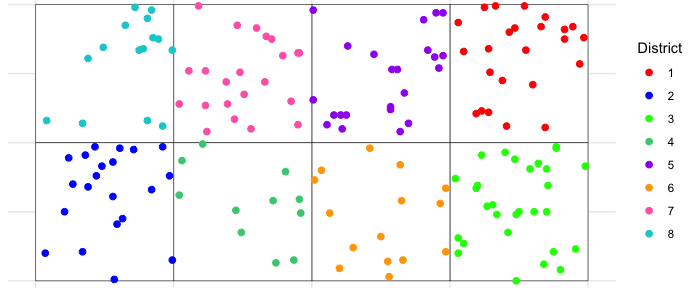
\includegraphics[width=0.80\textwidth]{figures/SpatialGridSetups/SampledPoints.png}
\caption{Example of simulated observation coordinates (n=160) on a 2x4 grid of clusters}
\label{figure:SampledPoints}
\end{figure}

\subsection{Simulation Evaluation Metrics}

Estimates for the baseline effect ($\alpha$), intervention effect ($\beta$), spillover effect ($\psi$), and spatial correlation parameter ($\rho$) were collected for each iteration of the simulation procedure for every treatment assignment combination. Considering the initial fixed simulation parameters, the following metrics are computed for estimation of the intervention effect for the evaluation of each set of simulation conditions.\\

% \begin{itemize}
%     \item $\textbf{Bias}$: a measure of how different the estimated parameter value is from the true parameter value. Small bias means that the parameter estimate is quite close to the true value.
%     \item $\textbf{Variance}$: a measure of the spread of a set of estimates from multiple simulation iterations. Smaller variance indicates that the estimates are tightly grouped together and large variance means that the estimates are spread out 
%     \item $\textbf{Mean Squared Error (MSE)}$: measures the average squared difference between each estimate and the true value of a parameter. Mean Squared Error combines variance to understand the consistency of a set of estimates as well as bias to understand any trend in deviation from the true value into a measure of estimation accuracy.
% \end{itemize}

\noindent $\textbf{Bias}$: a measure of how different the estimated parameter value is from the true parameter value. Small bias means that the parameter estimate is quite close to the true value.\\

\noindent $\textbf{Variance}$: a measure of the spread of a set of estimates from multiple simulation iterations. Smaller variance indicates that the estimates are tightly grouped together and large variance means that the estimates are spread out.\\

\noindent $\textbf{Mean Squared Error (MSE)}$: measures the average squared difference between each estimate and the true value of a parameter. Mean Squared Error combines variance to understand the consistency of a set of estimates as well as bias to understand any trend in deviation from the true value into a measure of estimation accuracy.\\

Mean Squared Error is the primary metric of consideration to understand the efficient estimation of the intervention effect under all simulation settings. The following subsections detail the findings from the simulation study, focusing on the Mean Squared Error (MSE), standard deviation (SD), and bias of the intervention effect ($\beta$) estimates under various conditions (simulation scenarios). The analysis compares Simple Random Sampling (SRS) and Block Stratified Sampling (BSS) across different spatial grid configurations, spillover effect magnitudes, spatial dependence levels, and spillover application types.

\subsection{Intervention Effect Estimates (2x4 grid)}

For the 2×4 spatial grid, the simulation results for the intervention effect estimates are presented in Table~\ref{table:InterventionEstimates2x4} and visually represented in Figure~\ref{figure:BetaMSE2x4Grouped}.

When spillover was applied to Control Clusters Only (TrtNoSpill), SRS generally exhibited higher MSE compared to BSS, particularly as the spillover effect ($\psi$) increased. For instance, with $\rho=0$ (no spatial dependence), SRS MSE ranged from $0.173$ ($\psi=0.5$) to $0.441$ ($\psi=0.8$), while BSS maintained very low MSE values (e.g., $0.008$ for $\psi=0.5$). Similarly, with $\rho=0.01$ (spatial dependence), SRS MSE increased from $0.304$ ($\psi=0.5$) to $0.573$ ($\psi=0.8$), whereas BSS showed MSE values ranging from $0.165$ to $0.569$. BSS consistently demonstrated smaller standard deviations compared to SRS under this spillover application type, indicating greater precision. SRS estimates generally showed negative bias, which increased in magnitude with higher $\psi$.

When spillover was applied to Intervention \& Control Clusters (TrtSpill), SRS generally showed lower MSE compared to BSS, especially in the absence of spatial dependence ($\rho=0$). For $\rho=0$, SRS MSE ranged from $0.008$ ($\psi=0.5$) to $0.019$ ($\psi=0.8$), while BSS MSE was consistently higher (e.g., $0.262$ for $\psi=0.5$). With spatial dependence ($\rho=0.01$), SRS still maintained lower MSE ($0.095$ to $0.162$) compared to BSS ($0.165$ to $0.569$). SRS also exhibited smaller standard deviations and bias magnitudes under this condition, suggesting better overall accuracy and precision.

Across both spillover application types for the 2×4 grid, the presence of spatial dependence ($\rho=0.01$) consistently led to higher MSE values for both sampling methods compared to scenarios without spatial dependence ($\rho=0$).

% --- Figure: Beta MSE for 2x4 (side by side) ---
% \begin{figure}[!ht]
%     \centering % Centers the entire block of minipages

%     % Left Column Figure
%     \begin{minipage}{0.45\textwidth} % Minipage for the left figure
%         \centering % Centers image within its minipage
%         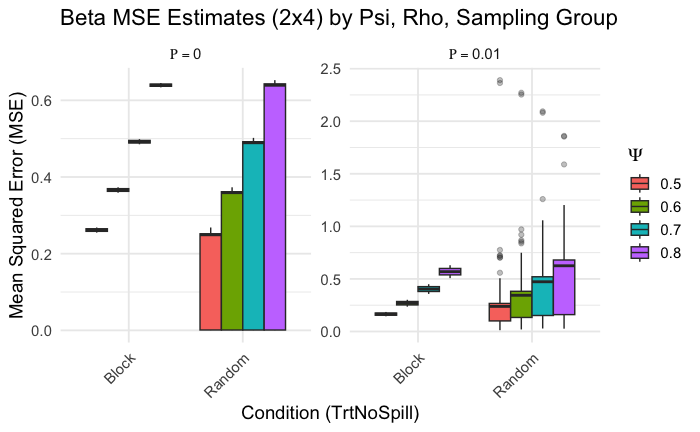
\includegraphics[width=\linewidth]{figures/BetaMSEresults/BetaMSEtrtNoSpill2x4.png}
%         % \caption{Intervention effect MSE for 2x4 cluster grid with spillover allowed only on control clusters}
%         % \label{figure:BetaMSEtrtNoSpill2x4}
%     \end{minipage}%\hspace*{\fill}%  <--- CRITICAL: Ensure NO actual newline character, blank line, or extra spaces between this '%' and the '\begin{minipage}' below. This entire sequence should be one continuous "line" in your .tex file.
%     \hfill % \hfill puts a flexible horizontal space between minipages
%     \begin{minipage}{0.45\textwidth} % Minipage for the right figure
%         \centering % Centers image within its minipage
%         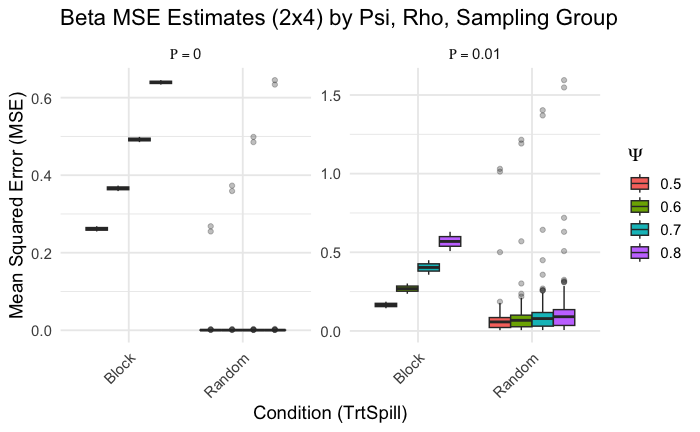
\includegraphics[width=\linewidth]{figures/BetaMSEresults/BetaMSEtrtSpill2x4.png}
%         % \caption{3x4 spatial grid of intervention (red) and control (blue) clusters assigned via Simple Random Sampling}
%         % \label{figure:BetaMSEtrtSpill2x4}
%     \end{minipage}

%     % Overall figure caption
%     \caption{Intervention effect MSE for 2x4 cluster grid with spillover allowed on control and intervention clusters}
%     \label{figure:BetaMSE2x4}
% \end{figure}

% --- Figure: Consolidated Intervention MSE for 2x4 grid ---
\begin{figure} [!ht]
\centering
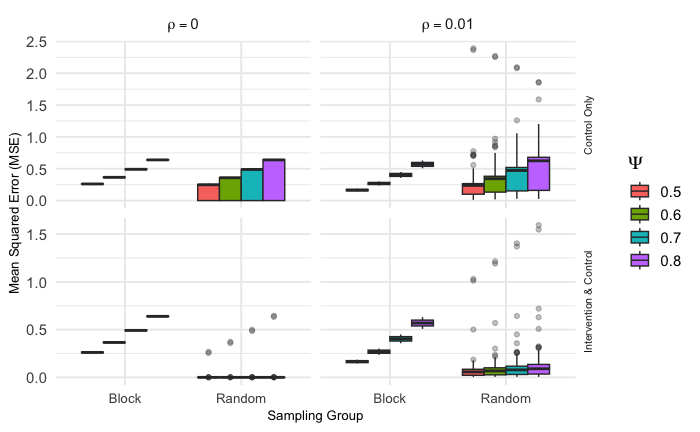
\includegraphics[width=0.80\textwidth]{figures/BetaMSEresults/MSE_Estimates_2x4.png}
\caption{Intervention effect MSE for 2x4 cluster grid grouped by spillover effect magnitude, spatial dependence, sampling design, and spillover application type}
\label{figure:BetaMSE2x4Grouped}
\end{figure}

% --- Table: Results for 2x4 Grid ---
% \begin{table}[ht!]
% \centering % Use \centering for better vertical spacing
% \begin{tabular}{ l c c ccc ccc } % 'l' for left-aligned, 'c' for center-aligned
%     \toprule % Top rule from booktabs package
%     \textbf{\makecell{Spillover \\ Application}} & \textbf{\makecell{Spatial \\ Dependence \\ ($\rho$)}} & \textbf{\makecell{Spillover \\ Effect \\ ($\psi$)}} & \multicolumn{3}{c}{\textbf{\makecell{Simple Random\\ Sampling}}} & \multicolumn{3}{c}{\textbf{\makecell{Block Stratified\\ Sampling}}} \\
%     \cmidrule(lr){4-6} \cmidrule(lr){7-9} % Partial rules for sub-headers
%     & & & MSE & SD & Bias & MSE & SD & Bias \\
%     \midrule % Mid rule from booktabs package
%     \multirow{8}{*}{\makecell{Control Only\\ Spillover}} & \multirow{4}{*}{\makecell{Yes ($0.01$)}} & 0.5 & 0.30384 & 0.40525 & -0.26984 & 0.16515 & 0.02943 & -0.34903 \\
%     & & 0.6 & 0.38161 & 0.40623 & -0.34198 & 0.26900 & 0.04620 & -0.47130 \\
%     & & 0.7 & 0.47105 & 0.41430 & -0.41415 & 0.40359 & 0.06531 & -0.59377 \\
%     & & 0.8 & 0.57345 & 0.43896 & -0.48647 & 0.56900 & 0.08672 & -0.71637 \\
%     \cmidrule(lr){2-9} % Horizontal line spanning from Spatial Dependence to the end
%     & \multirow{4}{*}{\makecell{No ($0.00$)}} & 0.5 & 0.17278 & 0.11696 & -0.34278 & 0.26160 & 0.00946 & -0.49594 \\
%     & & 0.6 & 0.24823 & 0.16834 & -0.41130 & 0.36608 & 0.00998 & -0.59661 \\
%     & & 0.7 & 0.33754 & 0.22914 & -0.47979 & 0.49203 & 0.00951 & -0.69728 \\
%     & & 0.8 & 0.44075 & 0.29940 & -0.54826 & 0.63946 & 0.00806 & -0.79795 \\
%     \midrule % Mid rule to separate spillover applications
%     \multirow{8}{*}{\makecell{Intervention \&\\ Control Spillover}} & \multirow{4}{*}{\makecell{Yes ($0.01$)}} & 0.5 & 0.09543 & 0.17615 & 0.03072 & 0.16515 & 0.02943 & -0.34903 \\
%     & & 0.6 & 0.11542 & 0.20822 & 0.02984 & 0.26900 & 0.04620 & -0.47130 \\
%     & & 0.7 & 0.13772 & 0.24225 & 0.02862 & 0.40359 & 0.06531 & -0.59377 \\
%     & & 0.8 & 0.16216 & 0.27871 & 0.02714 & 0.56900 & 0.08672 & -0.71637 \\
%     \cmidrule(lr){2-9}
%     & \multirow{4}{*}{\makecell{No ($0.00$)}} & 0.5 & 0.00790 & 0.04384 & -0.01400 & 0.26160 & 0.00946 & -0.49594 \\
%     & & 0.6 & 0.01090 & 0.06137 & -0.01679 & 0.36608 & 0.00998 & -0.59661 \\
%     & & 0.7 & 0.01450 & 0.08250 & -0.01964 & 0.49203 & 0.00951 & -0.69728 \\
%     & & 0.8 & 0.01872 & 0.10723 & -0.02255 & 0.63946 & 0.00806 & -0.79795 \\
%     \bottomrule % Bottom rule from booktabs package
% \end{tabular}
% \caption{SRS vs. BSS: Intervention Effect Error Estimates - 2x4 Spatial Grid Setting}
% \label{table:InterventionEstimates2x4}
% \end{table}

\begin{table}[ht!]
\centering
\begin{tabular}{l c c ccc ccc}
    \toprule
    \textbf{\makecell{Spillover \\ Application}} & \textbf{\makecell{Spatial \\ Dependence \\ ($\rho$)}} & \textbf{\makecell{Spillover \\ Effect \\ ($\psi$)}} & \multicolumn{3}{c}{\textbf{\makecell{Simple Random\\ Sampling}}} & \multicolumn{3}{c}{\textbf{\makecell{Block Stratified\\ Sampling}}} \\
    \cmidrule(lr){4-6} \cmidrule(lr){7-9}
    & & & MSE & \makecell{SD \\ ($\times 10$)} & Bias & MSE & \makecell{SD \\ ($\times 10$)} & Bias \\
    \midrule
    \multirow{8}{*}{\makecell{Control Only\\ Spillover}} & \multirow{4}{*}{\makecell{Yes ($0.01$)}} & 0.5 & 0.304 & 4.053 & -0.270 & 0.165 & 0.294 & -0.349 \\
    & & 0.6 & 0.382 & 4.062 & -0.342 & 0.269 & 0.462 & -0.471 \\
    & & 0.7 & 0.471 & 4.143 & -0.414 & 0.404 & 0.653 & -0.594 \\
    & & 0.8 & 0.573 & 4.390 & -0.486 & 0.569 & 0.867 & -0.716 \\
    \cmidrule(lr){2-9}
    & \multirow{4}{*}{\makecell{No ($0$)}} & 0.5 & 0.173 & 1.170 & -0.343 & 0.262 & 0.095 & -0.496 \\
    & & 0.6 & 0.248 & 1.683 & -0.411 & 0.366 & 0.100 & -0.597 \\
    & & 0.7 & 0.338 & 2.291 & -0.480 & 0.492 & 0.095 & -0.697 \\
    & & 0.8 & 0.441 & 2.994 & -0.548 & 0.639 & 0.081 & -0.798 \\
    \midrule
    \multirow{8}{*}{\makecell{Intervention \&\\ Control Spillover}} & \multirow{4}{*}{\makecell{Yes ($0.01$)}} & 0.5 & 0.095 & 1.762 & 0.031 & 0.165 & 0.294 & -0.349 \\
    & & 0.6 & 0.115 & 2.082 & 0.030 & 0.269 & 0.462 & -0.471 \\
    & & 0.7 & 0.138 & 2.423 & 0.029 & 0.404 & 0.653 & -0.594 \\
    & & 0.8 & 0.162 & 2.787 & 0.027 & 0.569 & 0.867 & -0.716 \\
    \cmidrule(lr){2-9}
    & \multirow{4}{*}{\makecell{No ($0$)}} & 0.5 & 0.008 & 0.438 & -0.014 & 0.262 & 0.095 & -0.496 \\
    & & 0.6 & 0.011 & 0.614 & -0.017 & 0.366 & 0.100 & -0.597 \\
    & & 0.7 & 0.015 & 0.825 & -0.020 & 0.492 & 0.095 & -0.697 \\
    & & 0.8 & 0.019 & 1.072 & -0.023 & 0.639 & 0.081 & -0.798 \\
    \bottomrule
\end{tabular}
\caption{SRS vs. BSS: Intervention Effect Error Estimates - 2x4 Spatial Grid Setting}
\label{table:InterventionEstimates2x4}
\end{table}

% \pagebreak

\subsection{Intervention Effect Estimates (3x3 grid)}

The results for the 3×3 spatial grid are summarized in Table~\ref{table:InterventionEstimates3x3} and Figure~\ref{figure:BetaMSE3x3Grouped}.

For the Control Clusters Only (TrtNoSpill) spillover application, BSS consistently yielded significantly lower MSE, SD, and bias compared to SRS. For instance, with $\rho=0$, BSS MSE was minimal (e.g., $0.001$ for $\psi=0.5$), while SRS MSE ranged from $0.092$ to $0.235$. This pattern held true with spatial dependence ($\rho=0.01$), where BSS MSE remained very low (e.g., $0.004$ for $\psi=0.5$), contrasting with SRS MSE values ranging from $0.259$ to $0.372$. SRS estimates consistently showed negative bias, increasing with $\psi$, while BSS bias was negligible.

In the Intervention \& Control Clusters (TrtSpill) spillover scenario, BSS continued to demonstrate superior performance with substantially lower MSE, SD, and bias compared to SRS. For $\rho=0$, BSS MSE was consistently around $0.0004$, whereas SRS MSE ranged from $0.002$ to $0.005$. With $\rho=0.01$, BSS MSE was also consistently very low (e.g., $0.039$ for $\psi=0.5$), while SRS MSE ranged from $0.103$ to $0.168$.

Similar to the 2×4 grid, the presence of spatial dependence ($\rho=0.01$) generally increased MSE for both sampling methods across both spillover application types for the 3×3 grid.

% --- Figure: Beta MSE for 3x3 (side by side) ---
% \begin{figure}[!ht]
%     \centering % Centers the entire block of minipages

%     % Left Column Figure
%     \begin{minipage}{0.45\textwidth} % Minipage for the left figure
%         \centering % Centers image within its minipage
%         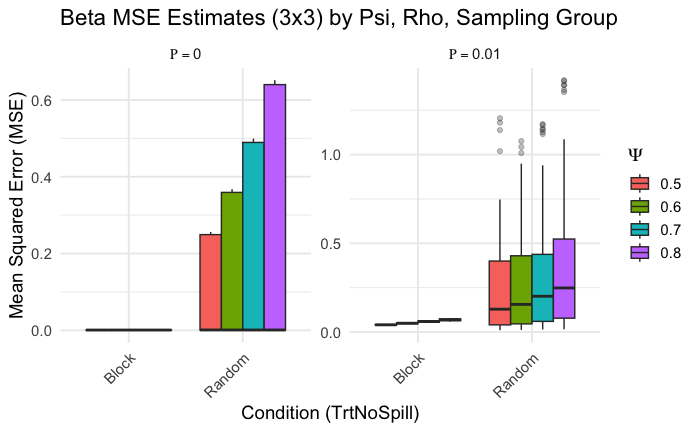
\includegraphics[width=\linewidth]{figures/BetaMSEresults/BetaMSEtrtNoSpill3x3.png}
%         % \caption{Intervention effect MSE for 3x3 cluster grid with spillover allowed only on control clusters}
%         % \label{figure:BetaMSEtrtNoSpill3x3}
%     \end{minipage}%\hspace*{\fill}%  <--- CRITICAL: Ensure NO actual newline character, blank line, or extra spaces between this '%' and the '\begin{minipage}' below. This entire sequence should be one continuous "line" in your .tex file.
%     \hfill % \hfill puts a flexible horizontal space between minipages
%     \begin{minipage}{0.45\textwidth} % Minipage for the right figure
%         \centering % Centers image within its minipage
%         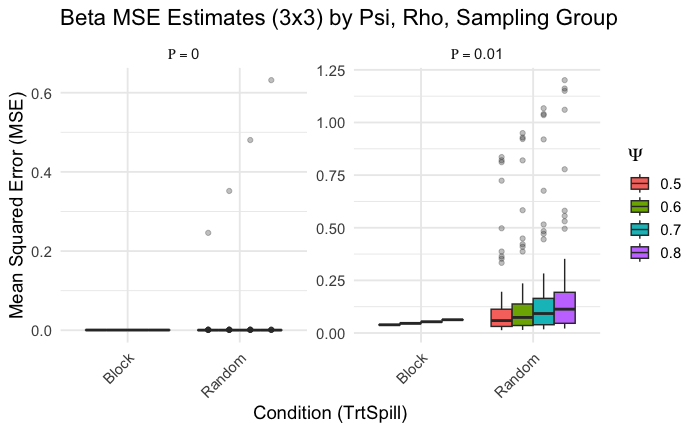
\includegraphics[width=\linewidth]{figures/BetaMSEresults/BetaMSEtrtSpill3x3.png}
%         % \caption{3x3 spatial grid of intervention (red) and control (blue) clusters assigned via Simple Random Sampling}
%         % \label{figure:BetaMSEtrtSpill3x3}
%     \end{minipage}

%     % Overall figure caption
%     \caption{Intervention effect MSE for 3x3 cluster grid with spillover allowed on control and intervention clusters}
%     \label{figure:BetaMSE3x3}
% \end{figure}

% --- Figure: Consolidated Intervention MSE for 3x3 grid ---
\begin{figure} [!ht]
\centering
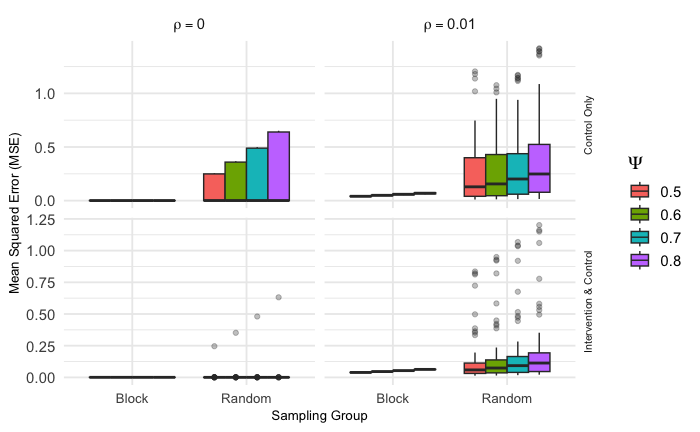
\includegraphics[width=0.80\textwidth]{figures/BetaMSEresults/MSE_Estimates_3x3.png}
\caption{Intervention effect MSE for 3x3 cluster grid grouped by spillover effect magnitude, spatial dependence, sampling design, and spillover application type}
\label{figure:BetaMSE3x3Grouped}
\end{figure}

% --- Table: Results for 3x3 Grid ---
% \begin{table}[ht!]
% \centering % Use \centering for better vertical spacing
% \begin{tabular}{ l c c ccc ccc } % 'l' for left-aligned, 'c' for center-aligned
%     \toprule % Top rule from booktabs package
%     \textbf{\makecell{Spillover \\ Application}} & \textbf{\makecell{Spatial \\ Dependence \\ ($\rho$)}} & \textbf{\makecell{Spillover \\ Effect \\ ($\psi$)}} & \multicolumn{3}{c}{\textbf{\makecell{Simple Random\\ Sampling}}} & \multicolumn{3}{c}{\textbf{\makecell{Block Stratified\\ Sampling}}} \\
%     \cmidrule(lr){4-6} \cmidrule(lr){7-9} % Partial rules for sub-headers
%     & & & MSE & SD & Bias & MSE & SD & Bias \\
%     \midrule % Mid rule from booktabs package
%     \multirow{8}{*}{\makecell{Control Only\\ Spillover}} & \multirow{4}{*}{\makecell{Yes ($0.01$)}} & 0.5 & 0.23379 & 0.25927 & -0.05399 & 0.04054 & 0.00440 & -0.01229 \\
%     & & 0.6 & 0.27638 & 0.28599 & -0.09229 & 0.04960 & 0.00797 & -0.01773 \\
%     & & 0.7 & 0.32234 & 0.32838 & -0.13104 & 0.05919 & 0.01144 & -0.02204 \\
%     & & 0.8 & 0.37154 & 0.38566 & -0.16998 & 0.06920 & 0.01446 & -0.02516 \\
%     \cmidrule(lr){2-9} % Horizontal line spanning from Spatial Dependence to the end
%     & \multirow{4}{*}{\makecell{No ($0.00$)}} & 0.5 & 0.09200 & 0.12071 & -0.18211 & 0.00069 & 0.00020 & 0.00280 \\
%     & & 0.6 & 0.13221 & 0.17397 & -0.21877 & 0.00070 & 0.00018 & 0.00289 \\
%     & & 0.7 & 0.17980 & 0.23701 & -0.25545 & 0.00071 & 0.00017 & 0.00298 \\
%     & & 0.8 & 0.23485 & 0.30992 & -0.29217 & 0.00071 & 0.00017 & 0.00305 \\
%     \midrule % Mid rule to separate spillover applications
%     \multirow{8}{*}{\makecell{Intervention \&\\ Control Spillover}} & \multirow{4}{*}{\makecell{Yes ($0.01$)}} & 0.5 & 0.10339 & 0.14801 & 0.07140 & 0.03899 & 0.00222 & -0.01899 \\
%     & & 0.6 & 0.12214 & 0.16878 & 0.08204 & 0.04588 & 0.00271 & -0.02000 \\
%     & & 0.7 & 0.14332 & 0.19051 & 0.09237 & 0.05355 & 0.00319 & -0.02101 \\
%     & & 0.8 & 0.16807 & 0.21492 & 0.10133 & 0.06303 & 0.00074 & -0.01899 \\
%     \cmidrule(lr){2-9}
%     & \multirow{4}{*}{\makecell{No ($0.00$)}} & 0.5 & 0.00233 & 0.02188 & -0.00357 & 0.00052 & 0.00044 & 0.00383 \\
%     & & 0.6 & 0.00318 & 0.03131 & -0.00437 & 0.00052 & 0.00044 & 0.00383 \\
%     & & 0.7 & 0.00420 & 0.04276 & -0.00518 & 0.00052 & 0.00044 & 0.00383 \\
%     & & 0.8 & 0.00541 & 0.05624 & -0.00600 & 0.00052 & 0.00044 & 0.00383 \\
%     \bottomrule % Bottom rule from booktabs package
% \end{tabular}
% \caption{SRS vs. BSS: Intervention Effect Error Estimates - 3x3 Spatial Grid Setting}
% \label{table:InterventionEstimates3x3}
% \end{table}

\begin{table}[ht!]
\centering
\begin{tabular}{l c c ccc ccc}
    \toprule
    \textbf{\makecell{Spillover \\ Application}} & \textbf{\makecell{Spatial \\ Dependence \\ ($\rho$)}} & \textbf{\makecell{Spillover \\ Effect \\ ($\psi$)}} & \multicolumn{3}{c}{\textbf{\makecell{Simple Random\\ Sampling}}} & \multicolumn{3}{c}{\textbf{\makecell{Block Stratified\\ Sampling}}} \\
    \cmidrule(lr){4-6} \cmidrule(lr){7-9}
    & & & MSE & \makecell{SD \\ ($\times 10$)} & Bias & MSE & \makecell{SD \\ ($\times 10$)} & Bias \\
    \midrule
    \multirow{8}{*}{\makecell{Control Only\\ Spillover}} & \multirow{4}{*}{\makecell{Yes ($0.01$)}} & 0.5 & 0.234 & 2.593 & -0.054 & 0.041 & 0.044 & -0.012 \\
    & & 0.6 & 0.276 & 2.860 & -0.092 & 0.050 & 0.080 & -0.018 \\
    & & 0.7 & 0.322 & 3.284 & -0.131 & 0.059 & 0.114 & -0.022 \\
    & & 0.8 & 0.372 & 3.857 & -0.170 & 0.069 & 0.145 & -0.025 \\
    \cmidrule(lr){2-9}
    & \multirow{4}{*}{\makecell{No ($0$)}} & 0.5 & 0.092 & 1.207 & -0.182 & 0.001 & 0.002 & 0.003 \\
    & & 0.6 & 0.132 & 1.740 & -0.219 & 0.001 & 0.002 & 0.003 \\
    & & 0.7 & 0.180 & 2.370 & -0.255 & 0.001 & 0.002 & 0.003 \\
    & & 0.8 & 0.235 & 3.099 & -0.292 & 0.001 & 0.002 & 0.003 \\
    \midrule
    \multirow{8}{*}{\makecell{Intervention \&\\ Control Spillover}} & \multirow{4}{*}{\makecell{Yes ($0.01$)}} & 0.5 & 0.103 & 1.480 & 0.071 & 0.039 & 0.022 & -0.019 \\
    & & 0.6 & 0.122 & 1.688 & 0.082 & 0.046 & 0.027 & -0.020 \\
    & & 0.7 & 0.143 & 1.905 & 0.092 & 0.054 & 0.032 & -0.021 \\
    & & 0.8 & 0.168 & 2.149 & 0.101 & 0.063 & 0.007 & -0.019 \\
    \cmidrule(lr){2-9}
    & \multirow{4}{*}{\makecell{No ($0$)}} & 0.5 & 0.002 & 0.219 & -0.004 & 0.001 & 0.004 & 0.004 \\
    & & 0.6 & 0.003 & 0.313 & -0.004 & 0.001 & 0.004 & 0.004 \\
    & & 0.7 & 0.004 & 0.428 & -0.005 & 0.001 & 0.004 & 0.004 \\
    & & 0.8 & 0.005 & 0.562 & -0.006 & 0.001 & 0.004 & 0.004 \\
    \bottomrule
\end{tabular}
\caption{SRS vs. BSS: Intervention Effect Error Estimates - 3x3 Spatial Grid Setting}
\label{table:InterventionEstimates3x3}
\end{table}

% \pagebreak

\subsection{Intervention Effect Estimates (3x4 grid)}

Table~\ref{table:InterventionEstimates3x4} and Figure~\ref{figure:BetaMSE3x4Grouped} present the intervention effect estimates for the 3×4 spatial grid.

Under the Control Clusters Only (TrtNoSpill) spillover condition, BSS consistently outperformed SRS in terms of MSE, SD, and bias. With $\rho=0$, BSS MSE was extremely low (e.g., $0.0004$ for $\psi=0.5$), while SRS MSE ranged from $0.034$ to $0.219$. This trend persisted with $\rho=0.01$, where BSS MSE remained low (e.g., $0.035$ for $\psi=0.5$), compared to SRS MSE ranging from $0.120$ to $0.204$. SRS estimates generally showed a small positive or negative bias, while BSS bias was consistently negligible.

For the Intervention \& Control Clusters (TrtSpill) spillover application, BSS again showed superior performance with lower MSE, SD, and bias. With $\rho=0$, BSS MSE was consistently around $0.0003$, while SRS MSE ranged from $0.0007$ to $0.029$. With $\rho=0.01$, BSS MSE was also low (e.g., $0.223$ for $\psi=0.5$), while SRS MSE ranged from $0.112$ to $0.190$.

Across all grid sizes and conditions, increasing the spillover effect magnitude ($\psi$) generally led to an increase in MSE for both sampling methods. The presence of spatial dependence ($\rho=0.01$) consistently resulted in higher MSE for both SRS and BSS compared to scenarios without spatial dependence ($\rho=0$). While SRS sometimes showed lower MSE when spillover was applied to both intervention and control clusters, BSS consistently demonstrated lower variance and often lower bias, particularly when spillover was restricted to control clusters only. This highlights that BSS provides more consistent estimates, even if SRS might occasionally yield a lower average error depending on the specific spillover dynamics.

% --- Figure: Beta MSE for 3x4 (side by side) ---
% \begin{figure}[!ht]
%     \centering % Centers the entire block of minipages

%     % Left Column Figure
%     \begin{minipage}{0.45\textwidth} % Minipage for the left figure
%         \centering % Centers image within its minipage
%         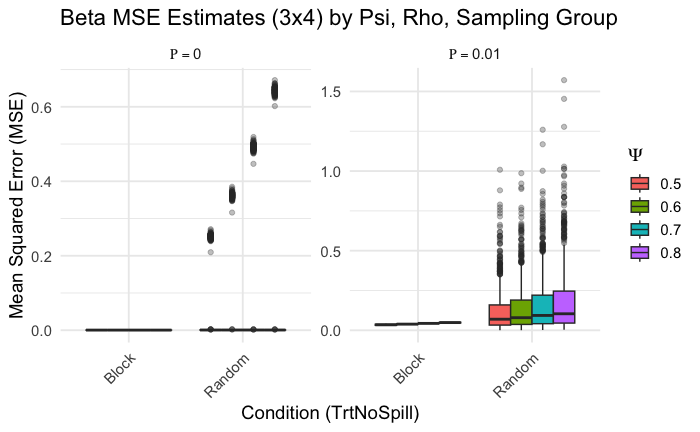
\includegraphics[width=\linewidth]{figures/BetaMSEresults/BetaMSEtrtNoSpill3x4.png}
%         % \caption{Intervention effect MSE for 3x4 cluster grid with spillover allowed only on control clusters}
%         % \label{figure:BetaMSEtrtNoSpill3x4}
%     \end{minipage}%\hspace*{\fill}%  <--- CRITICAL: Ensure NO actual newline character, blank line, or extra spaces between this '%' and the '\begin{minipage}' below. This entire sequence should be one continuous "line" in your .tex file.
%     \hfill % \hfill puts a flexible horizontal space between minipages
%     \begin{minipage}{0.45\textwidth} % Minipage for the right figure
%         \centering % Centers image within its minipage
%         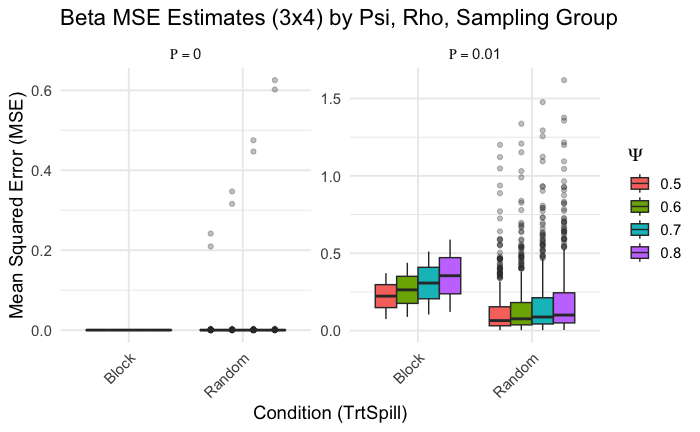
\includegraphics[width=\linewidth]{figures/BetaMSEresults/BetaMSEtrtSpill3x4.png}
%         % \caption{3x4 spatial grid of intervention (red) and control (blue) clusters assigned via Simple Random Sampling}
%         % \label{figure:BetaMSEtrtSpill3x4}
%     \end{minipage}

%     % Overall figure caption
%     \caption{Intervention effect MSE for 3x4 cluster grid with spillover allowed on control and intervention clusters}
%     \label{figure:BetaMSE3x4}
% \end{figure}

% --- Figure: Consolidated Intervention MSE for 3x4 grid ---
\begin{figure} [!ht]
\centering
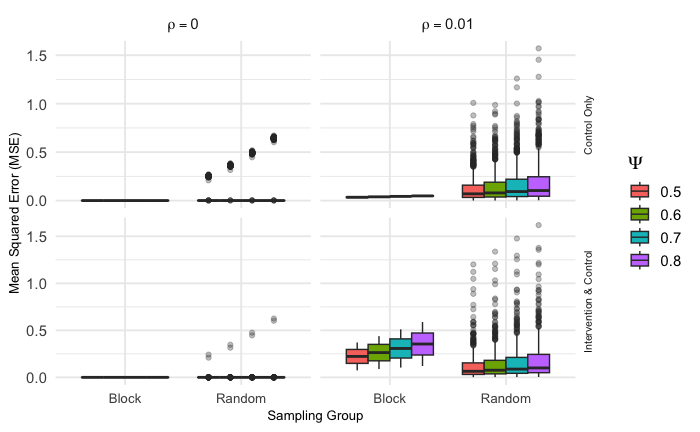
\includegraphics[width=0.80\textwidth]{figures/BetaMSEresults/MSE_Estimates_3x4.png}
\caption{Intervention effect MSE for 3x4 cluster grid grouped by spillover effect magnitude, spatial dependence, sampling design, and spillover application type}
\label{figure:BetaMSE3x4Grouped}
\end{figure}

% --- Table: Results for 3x4 Grid ---
% \begin{table}[ht!]
% \centering % Use \centering for better vertical spacing
% \begin{tabular}{ l c c ccc ccc } % 'l' for left-aligned, 'c' for center-aligned
%     \toprule % Top rule from booktabs package
%     \textbf{\makecell{Spillover \\ Application}} & \textbf{\makecell{Spatial \\ Dependence \\ ($\rho$)}} & \textbf{\makecell{Spillover \\ Effect \\ ($\psi$)}} & \multicolumn{3}{c}{\textbf{\makecell{Simple Random\\ Sampling}}} & \multicolumn{3}{c}{\textbf{\makecell{Block Stratified\\ Sampling}}} \\
%     \cmidrule(lr){4-6} \cmidrule(lr){7-9} % Partial rules for sub-headers
%     & & & MSE & SD & Bias & MSE & SD & Bias \\
%     \midrule % Mid rule from booktabs package
%     \multirow{8}{*}{\makecell{Control Only\\ Spillover}} & \multirow{4}{*}{\makecell{Yes ($0.01$)}} & 0.5 & 0.12009 & 0.13244 & 0.03254 & 0.03463 & 0.00963 & -0.15200 \\
%     & & 0.6 & 0.13800 & 0.14807 & 0.02057 & 0.03881 & 0.00505 & -0.16651 \\
%     & & 0.7 & 0.15902 & 0.17166 & 0.00943 & 0.04345 & 0.00011 & -0.18039 \\
%     & & 0.8 & 0.18330 & 0.20387 & -0.00075 & 0.04842 & 0.00561 & -0.19332 \\
%     \cmidrule(lr){2-9} % Horizontal line spanning from Spatial Dependence to the end
%     & \multirow{4}{*}{\makecell{No ($0.00$)}} & 0.5 & 0.03425 & 0.08554 & -0.06751 & 0.00036 & 0.00022 & -0.00571 \\
%     & & 0.6 & 0.04905 & 0.12318 & -0.08097 & 0.00036 & 0.00022 & -0.00563 \\
%     & & 0.7 & 0.06666 & 0.16769 & -0.09444 & 0.00035 & 0.00020 & -0.00555 \\
%     & & 0.8 & 0.08678 & 0.21912 & -0.10791 & 0.00034 & 0.00016 & -0.00553 \\
%     \midrule % Mid rule to separate spillover applications
%     \multirow{8}{*}{\makecell{Intervention \&\\ Control Spillover}} & \multirow{4}{*}{\makecell{Yes ($0.01$)}} & 0.5 & 0.11193 & 0.12873 & 0.02201 & 0.22286 & 0.20995 & -0.41486 \\
%     & & 0.6 & 0.13069 & 0.14762 & 0.02096 & 0.26343 & 0.24750 & -0.45154 \\
%     & & 0.7 & 0.15112 & 0.16817 & 0.01963 & 0.30741 & 0.28774 & -0.48833 \\
%     & & 0.8 & 0.17323 & 0.19046 & 0.01810 & 0.35475 & 0.33060 & -0.52516 \\
%     \cmidrule(lr){2-9}
%     & \multirow{4}{*}{\makecell{No ($0.00$)}} & 0.5 & 0.00073 & 0.01051 & -0.00126 & 0.00028 & 0.00004 & -0.00251 \\
%     & & 0.6 & 0.00096 & 0.01542 & -0.00149 & 0.00029 & 0.00004 & -0.00241 \\
%     & & 0.7 & 0.00124 & 0.02143 & -0.00172 & 0.00030 & 0.00005 & -0.00232 \\
%     & & 0.8 & 0.00158 & 0.02853 & -0.00194 & 0.00031 & 0.00005 & -0.00224 \\
%     \bottomrule % Bottom rule from booktabs package
% \end{tabular}
% \caption{SRS vs. BSS: Intervention Effect Error Estimates - 3x4 Spatial Grid Setting}
% \label{table:InterventionEstimates3x4}
% \end{table}

\begin{table}[ht!]
\centering
\begin{tabular}{l c c ccc ccc}
    \toprule
    \textbf{\makecell{Spillover \\ Application}} & \textbf{\makecell{Spatial \\ Dependence \\ ($\rho$)}} & \textbf{\makecell{Spillover \\ Effect \\ ($\psi$)}} & \multicolumn{3}{c}{\textbf{\makecell{Simple Random\\ Sampling}}} & \multicolumn{3}{c}{\textbf{\makecell{Block Stratified\\ Sampling}}} \\
    \cmidrule(lr){4-6} \cmidrule(lr){7-9}
    & & & MSE & \makecell{SD \\($\times 100$)} & Bias & \makecell{MSE \\($\times 10$)} & \makecell{SD \\($\times 100$)} & Bias \\
    \midrule
    \multirow{8}{*}{\makecell{Control Only\\ Spillover}} & \multirow{4}{*}{\makecell{Yes ($0.01$)}} & 0.5 & 0.120 & 13.244 & 0.033 & 0.346 & 0.963 & -0.152 \\
    & & 0.6 & 0.138 & 14.807 & 0.021 & 0.388 & 0.505 & -0.167 \\
    & & 0.7 & 0.159 & 17.166 & 0.009 & 0.435 & 0.011 & -0.180 \\
    & & 0.8 & 0.183 & 20.387 & -0.001 & 0.484 & 0.561 & -0.193 \\
    \cmidrule(lr){2-9}
    & \multirow{4}{*}{\makecell{No ($0$)}} & 0.5 & 0.034 & 8.554 & -0.068 & 0.004 & 0.022 & -0.006 \\
    & & 0.6 & 0.049 & 12.318 & -0.081 & 0.004 & 0.022 & -0.006 \\
    & & 0.7 & 0.067 & 16.769 & -0.094 & 0.004 & 0.020 & -0.006 \\
    & & 0.8 & 0.087 & 21.912 & -0.108 & 0.003 & 0.016 & -0.006 \\
    \midrule
    \multirow{8}{*}{\makecell{Intervention \&\\ Control Spillover}} & \multirow{4}{*}{\makecell{Yes ($0.01$)}} & 0.5 & 0.112 & 12.873 & 0.022 & 2.229 & 20.995 & -0.415 \\
    & & 0.6 & 0.131 & 14.762 & 0.021 & 2.634 & 24.750 & -0.452 \\
    & & 0.7 & 0.151 & 16.817 & 0.020 & 3.074 & 28.774 & -0.488 \\
    & & 0.8 & 0.173 & 19.046 & 0.018 & 3.548 & 33.060 & -0.525 \\
    \cmidrule(lr){2-9}
    & \multirow{4}{*}{\makecell{No ($0$)}} & 0.5 & 0.001 & 1.051 & -0.001 & 0.003 & 0.004 & -0.003 \\
    & & 0.6 & 0.001 & 1.542 & -0.001 & 0.003 & 0.004 & -0.002 \\
    & & 0.7 & 0.001 & 2.143 & -0.002 & 0.003 & 0.005 & -0.002 \\
    & & 0.8 & 0.002 & 2.853 & -0.002 & 0.003 & 0.005 & -0.002 \\
    \bottomrule
\end{tabular}
\caption{SRS vs. BSS: Intervention Effect Error Estimates - 3x4 Spatial Grid Setting}
\label{table:InterventionEstimates3x4}
\end{table}

% \pagebreak

% \subsection{Intervention Effect Estimates (Control Only Spillover)}

% \begin{figure} [!ht]
% \centering
% 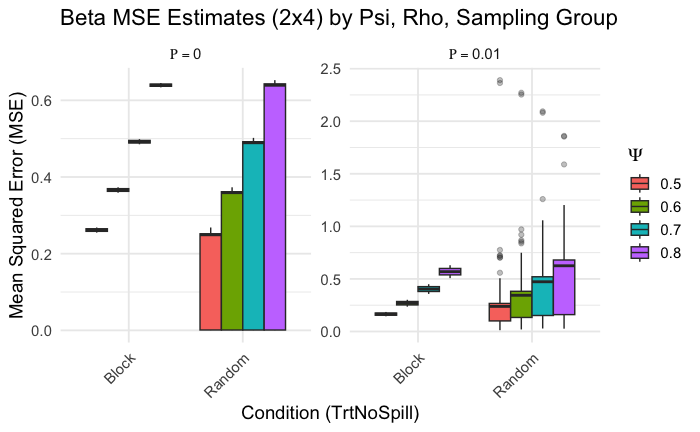
\includegraphics[width=0.60\textwidth]{figures/BetaMSEresults/BetaMSEtrtNoSpill2x4.png}
% \caption{Intervention effect MSE for 2x4 cluster grid with spillover allowed only on control clusters}
% \label{figure:BetaMSEtrtNoSpill2x4}
% \end{figure}

% \begin{figure} [!ht]
% \centering
% 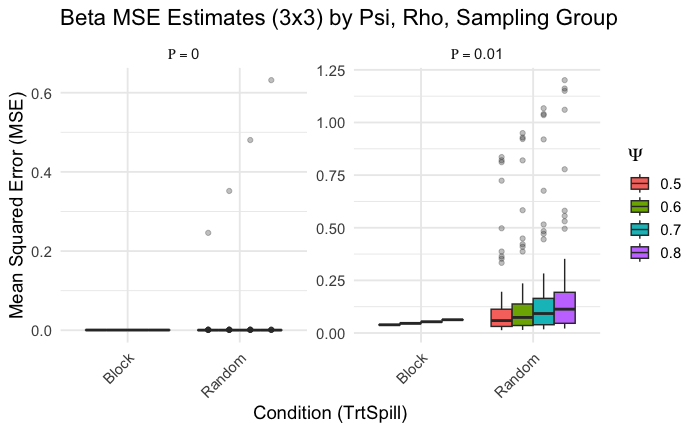
\includegraphics[width=0.60\textwidth]{figures/BetaMSEresults/BetaMSEtrtSpill3x3.png}
% \caption{Intervention effect MSE for 3x3 cluster grid with spillover allowed only on control clusters}
% \label{figure:BetaMSEtrtSpill3x3}
% \end{figure}

% \begin{figure} [!ht]
% \centering
% 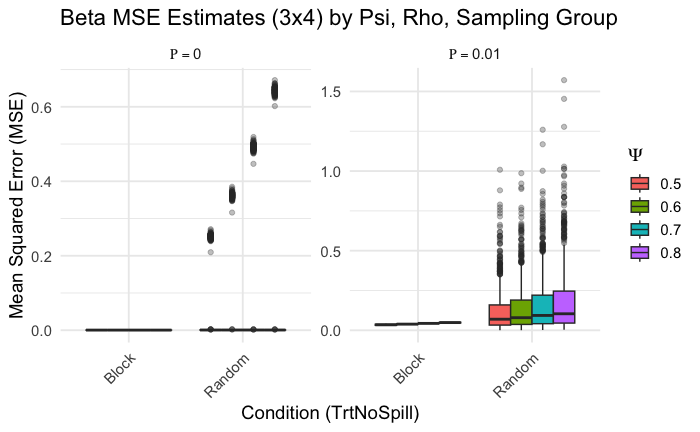
\includegraphics[width=0.60\textwidth]{figures/BetaMSEresults/BetaMSEtrtNoSpill3x4.png}
% \caption{Intervention effect MSE for 3x4 cluster grid with spillover allowed only on control clusters}
% \label{figure:BetaMSEtrtNoSpill3x4}
% \end{figure}

% \subsection{Intervention Effect Estimates (Intervention \& Control Spillover)}

% \begin{figure} [!ht]
% \centering
% 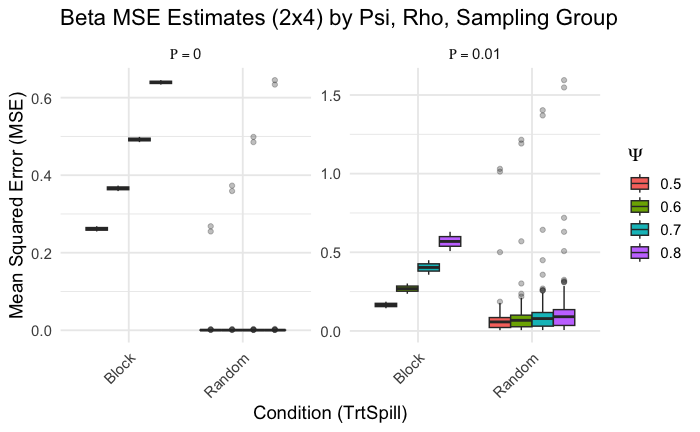
\includegraphics[width=0.60\textwidth]{figures/BetaMSEresults/BetaMSEtrtSpill2x4.png}
% \caption{Intervention effect MSE for 2x4 cluster grid with spillover allowed on control and intervention clusters}
% \label{figure:BetaMSEtrtSpill2x4}
% \end{figure}

% \begin{figure} [!ht]
% \centering
% 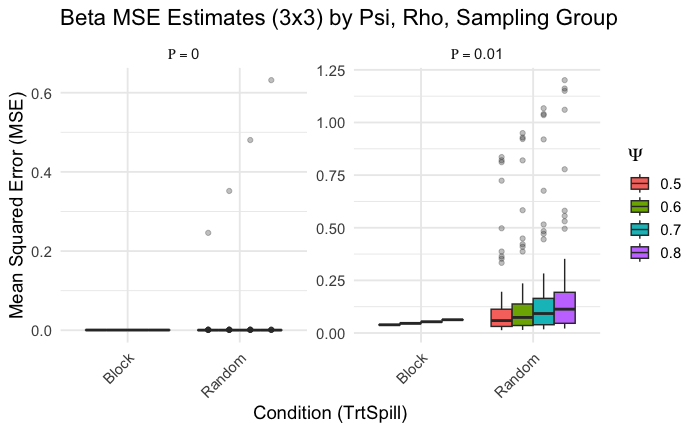
\includegraphics[width=0.60\textwidth]{figures/BetaMSEresults/BetaMSEtrtSpill3x3.png}
% \caption{Intervention effect MSE for 3x3 cluster grid with spillover allowed on control and intervention clusters}
% \label{figure:BetaMSEtrtSpill3x3}
% \end{figure}

% \begin{figure} [!ht]
% \centering
% 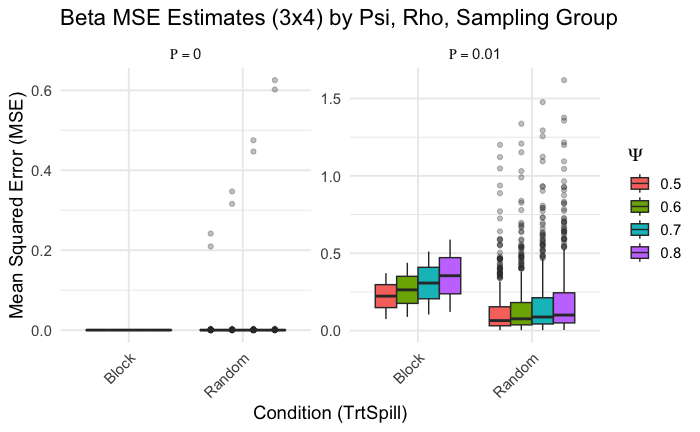
\includegraphics[width=0.60\textwidth]{figures/BetaMSEresults/BetaMSEtrtSpill3x4.png}
% \caption{Intervention effect MSE for 3x4 cluster grid with spillover allowed on control and intervention clusters}
% \label{figure:BetaMSEtrtSpill3x4}
% \end{figure}

% \subsection{Comparison of Methods}

% --- GA Study APPLICATION (application in practice) ---
\section{Application}

The findings from our simulation study provide relevant insights for investigators designing CRTs in real-world applications where spatial dependence and spillover effects are present and must be accounted for. In this case, a pair of studies in development that we consider involve the North Carolina Department of Adult Correction. The structure of correctional systems, particularly community supervision, often involves geographically clustered units where staff from different clusters may interact and regional similarities can influence outcomes. The investigators leading these studies desire recommendations for treatment assignment methodology regarding the spatially clustered nature of their design.

\subsection{Background of Probation in North Carolina}

The North Carolina Department of Adult Correction Division of Community Supervision (NC DCS) provides a clear example of a spatially structured organization, making it an ideal context for applying our research. The NC DCS is organized into four geographic Divisions numbered 1 through 4 from East to West, which are subdivided into 30 Districts that make up the entirety of the state. Each district is composed of one or more counties. If there is more than one county in the district, the counties are adjacent, but some districts are composed of only a singular county. In these districts, Probation and Parole Officers (PPOs) supervise individuals at the county level and are themselves managed by Chief Probation/Parole Officers (CPPOs) and Judicial District Managers (JDMs) who oversee districts. Each division (composed of multiple districts) is managed by a Judicial Division Director (JD Dir) as well. A map of the segmentation of each division and district is presented in Figure~\ref{figure:NCDCS_map}.

\begin{figure} [!ht]
\centering
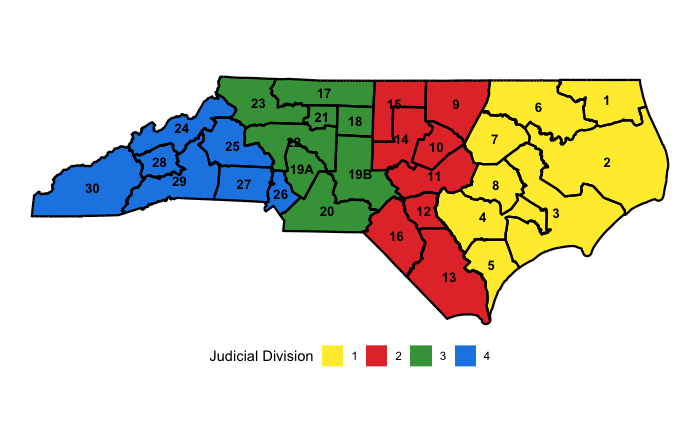
\includegraphics[width=0.80\textwidth]{figures/Applications/NC_DCS_Map_NoCounties.png}
\caption{The North Carolina Department of Adult Correction Division of Community Supervision map is segmented into 30 judicial districts that are grouped into 4 judicial divisions.}
\label{figure:NCDCS_map}
\end{figure}

This geographic and administrative structure means that Chiefs and Judicial District Managers (JDMs) often span multiple units and counties, creating a direct channel for spillover effects among regions under their supervision. For instance, if leadership views an intervention in one county favorably, they may implement its components in other counties under their jurisdiction, even if those areas were not assigned the intervention. Furthermore, adjacent counties within the same region often share demographic characteristics, labor market conditions, and similar judicial cultures, as well as the same managed care organizations and treatment providers, leading to spatial dependence in probation outcomes. The choice of treatment assignment sampling strategy in this context is non-trivial when considering potential options of either simple random sampling (SRS) or block-stratified sampling (BSS). Selection of the appropriate treatment sampling strategy may yield beneficial downstream outcomes when considering the error of intervention \& spillover estimates.

\subsection{Case 1: Trauma-Informed and Engaged Supervision}

One proposed study involves implementing a trauma-informed supervision model for PPOs managing specialty caseloads like domestic violence, sex offender, or gang affiliated cases. The intervention consists of intensive training and follow-up sessions delivered to cohorts of PPOs and CPPOs. The primary outcomes would be changes in officer knowledge and attitudes, as well as impacts on individuals under their supervision. The key design decision for this study is the unit of randomization. Randomizing at the PPO level is not feasible due to the high likelihood of spillover within a county office. Therefore, a cluster randomized design at the county or district level is necessary. This cluster randomization decision is also supported by agency-related logistics in addition to considerations for spillover. Original plans for a similar study, acknowledging the risk of contamination between adjacent units, considered randomization at the district level specifically to minimize spillover. This scenario directly reflects the conditions modeled in our simulation, where the effectiveness of an intervention in one cluster may influence outcomes in neighboring control clusters where an intervention is not applied.

\subsection{Case 2: Testing an implementation strategy for specialty mental health probation}

Another study proposal aims to test a strategy for improving the implementation of Specialty Mental Health Probation (SMHP). The intervention involves enhancing collaboration between PPOs and community-based behavioral health service providers through cross-training sessions and joint treatment team meetings. The primary outcome is improved collaboration, with secondary outcomes related to treatment engagement for individuals on probation. This case presents a more complex spatial challenge. In addition to the geographic proximity of probation districts, the behavioral health system in North Carolina is managed by four large Managed Care Organizations (MCOs), each responsible for a different coverage area. Some service provider agencies are large, operating in multiple counties and potentially across different MCO regions. This creates multiple, overlapping layers of potential spillover. Figure~\ref{figure:NCMCO_map} presents a map of which counties in the state that each MCO operates. An intervention implemented in one county could be adopted by a provider and informally carried into a neighboring control county, or an MCO could promote a similar initiative, confounding the study's results. This complex spatial linkage underscores the importance of a robust treatment assignment strategy in order to efficiently estimate the impact of the intervention.

\begin{figure} [!ht]
\centering
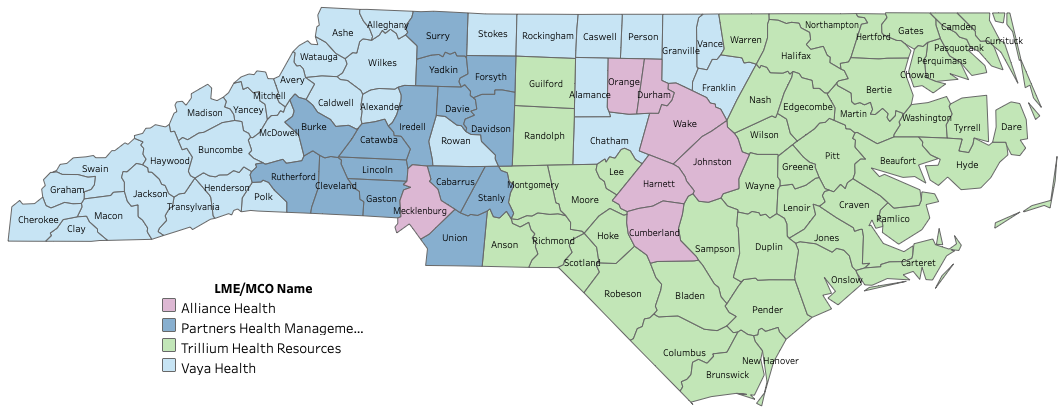
\includegraphics[width=0.80\textwidth]{figures/Applications/NC_MCO_Map.png}
\caption{Map of Local Management Entity/Managed Care Organizations (LME/MCOs) for each county in the state of North Carolina. There are 4 LME/MCOs of which one operates in each of the 100 counties of the state.}
\label{figure:NCMCO_map}
\end{figure}

\subsection{Recommendations for treatment assignment}
% Simulation comparison of SRS vs. BSS & interpretation
The results of our simulation study indicate a clear trade-off: we previously concluded that Simple Random Sampling (SRS) reduces the average mean squared error (MSE) across many randomizations (intervention/control combinations), while Block Stratified Sampling (BSS) reduces the variance of the error although it is not minimized. Put simply, BSS is less likely to produce a ``perfect" assignment by chance but is also robust against a ``worst-case" assignment that could render the study results invalid. For both case studies presented, Block Stratified Sampling (BSS) is the recommended approach.

% Recommendation & rationale for study 1
In Case 1 (Trauma-Informed Supervision), a simple random assignment of districts could, by chance, result in a geographic imbalance, concentrating treated districts in one part of the state. This would confound the intervention effect with regional characteristics. A more robust design would be to stratify by the four state divisions and randomize districts to intervention and control conditions within each division with a block stratification strategy. This ensures geographic balance and leverages the finding that BSS minimizes estimation variance, providing a more stable and defensible estimate of the intervention effect.

%ERecommendation & rationale for study 2 (EDIT THIS SECTION!)
In Case 2 (SMHP Implementation), the rationale for BSS is even stronger due to the complex potential for spillover. A simple random assignment of counties would ignore the significant structural influence of the MCOs. The most effective design would be to stratify by MCO coverage area, randomizing counties to the implementation strategy (intervention) or control condition within each MCO. This approach directly controls for the significant confounding variable of MCO-level policies and provider networks. However, some challenges with this MCO stratification do persist. For example, it's possible that a county is selected for the intervention and is supervised by a CPPO or even a judicial district manager that oversees a control group county. Furthermore, multiple service providers may serve a given county in the coverage area of an MCO and it is possible that multiple service providers begin team meetings. Another consideration is that some service providers are very large and have offices around the state and contract with more than one MCO. Based on this, we must consider potential spillover if after participating in a treatment team meeting, a service provider intends initiate those practices in another part of the state. Given the high risk of contamination, the robustness of BSS in minimizing error variance makes it the most prudent choice for achieving a reliable effect estimate. While SRS might achieve a lower MSE (intervention error estimate) in theory, the risk of a single, poorly distributed randomization in a complex, real-world setting outweighs the potential benefit. Therefore, it is wise to proceed with a sampling strategy that aims to manage estimation error with minimal variation.

% Describes sample BSS figure
A representation of this Block Stratification sampling strategy where we ``block" treatment and control districts together with an effort to isolate districts of a particular intervention status from each other is shown in Figure~\ref{figure:recommendation_map}. Note that across the entire map of the state and specifically in Judicial Division 1 (easternmost region) that when possible districts of the same intervention status are isolated from each other. When districts share a border with multiple other districts, this sampling method ensures that treatment districts are isolated from other treatment districts as best as possible.

\begin{figure} [!ht]
\centering
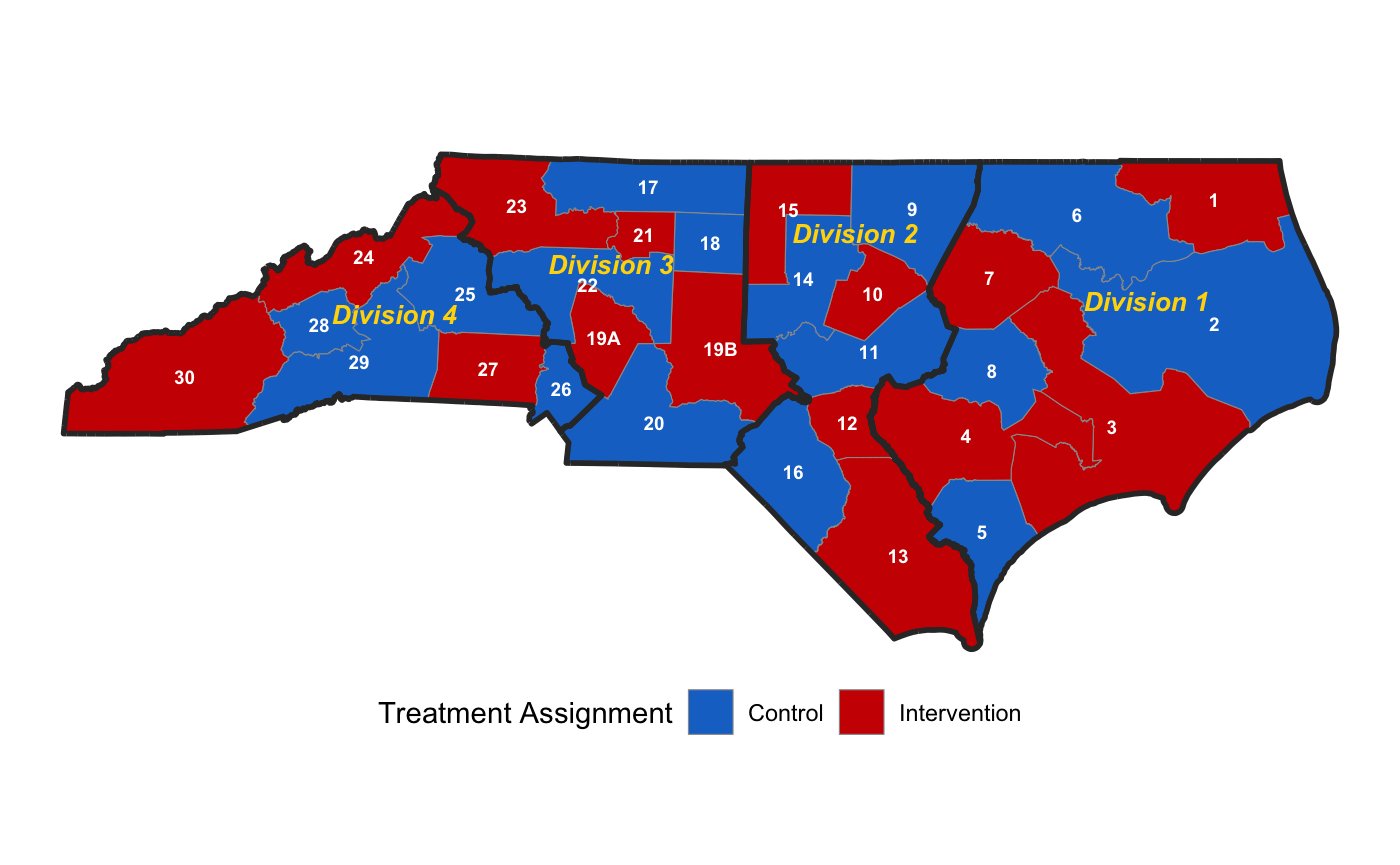
\includegraphics[width=0.80\textwidth]{figures/Applications/BSS_Assignments_NC_Map_Applications_Text_Labels.png}
\caption{Map of North Carolina with example block stratified sampling intervention assignments for each judicial district under consideration. Districts are assigned to either treatment (red) or control (blue).}
\label{figure:recommendation_map}
\end{figure}

% --- DISCUSSION ---
\section{Discussion}

\subsection{Relevance of results}

This simulation study provides insights into the efficiency of treatment assignment methodologies in spatial cluster randomized trials (CRTs) when considering spillover effects and spatial dependence. A primary contribution of this work is the direct comparison between Simple Random Sampling (SRS) and Block Stratified Sampling (BSS) across various scenarios, offering practical guidance for investigators designing such trials. 

Our findings show a clear relationship between the magnitude of spillover effects and the estimation error of the intervention effect. As the spillover effect ($\psi$) increases, the Mean Squared Error (MSE) for the intervention effect ($\beta$) generally rises, regardless of the sampling method or the presence of spatial dependence. This highlights the importance of accounting for spillover effects, as their increasing influence can diminish the accuracy of intervention effect estimates. The results indicate that randomly selected treatment assignments lead to reduced average error (lower bias) when estimating intervention effects, while block stratified treatment assignments consistently result in reduced variation (lower variance) among a series of estimates. This suggests a trade-off: SRS provides a more accurate central estimate on average, whereas BSS offers greater precision and consistency across repeated trials, potentially with higher bias. 

The study also clarifies the impact of spatial dependence ($\rho$) on intervention effect estimation error. The presence of even a small degree of spatial dependence (e.g., $\rho=0.01$) generally increased MSE for both sampling methods. This indicates that spatial correlation among observations can impede the accurate estimation of intervention effects if not managed during the design phase. The observed patterns across different spatial grid dimensions (2×4, 3×3, and 3×4) support these conclusions, demonstrating the consistency of the findings across varying spatial configurations. 

The investigation into cluster spillover restrictions (spillover to control clusters only vs. spillover to both control and intervention clusters) also identified important differences. When spillover was restricted to control clusters only, the MSE for the intervention effect was higher for SRS compared to BSS, particularly with increasing spillover magnitude. Conversely, when spillover was permitted for both control and intervention clusters, SRS often exhibited lower MSE, especially when spatial dependence was absent. This understanding of spillover application types provides investigators with a more precise basis for selecting a sampling strategy that aligns with their specific hypotheses regarding how an intervention's effects might propagate.

It is also insightful to note that for each simulation grid setup (2×4, 3×3, and 3×4), there are 7 different treatment assignment combinations that are the overall ``optimal" combination for at least one of the simulation scenarios in terms of MSE of the intervention effect estimate. It appears that the optimal treatment combination shifts as the components of each simulation scenario are adjusted and there is no consistent treatment combination from the Simple Random Sampling strategy that is optimal. This serves as further evidence to suggest that it is prudent to recommend the Block Stratified Sampling strategy because it provides results that consistently exhibit minimal MSE of the intervention effect estimate although the BSS treatment combinations are never the absolute best case in terms of MSE for any given simulation scenario. By implementing a BSS strategy, investigators will consistently obtain strong estimates of the intervention effect (although not the best for any specific single case) under the conditions of the spatial autoregressive (SAR) model.

In summary, this study offers a comparison of two opposing sampling methodologies in spatial CRTs. The patterns observed regarding spillover magnitude, spatial dependence, and spillover application types provide practical information for investigators. They must consider the goal of an unbiased average estimate (favored by SRS) versus the need for consistent, low-variance estimates (achieved with BSS), especially when designing studies where spillover effects are expected.

\subsection{Limitations}

While this simulation study provides valuable insights, it is important to acknowledge a few key limitations that may affect the generalizability and scope of its findings. The study encountered issues related to multicollinearity between the direct (intervention) and indirect (spillover) effects. In some spatial configurations and with specific spillover magnitudes, high correlation between the $x_i$ (intervention indicator) and $z_i$ (spillover indicator) variables in the spatial autoregressive model (Equation~\ref{Equation:SARmodel}) could lead to instability in parameter estimates. While the SAR model addresses spatial relationships, extreme collinearity can still impact the precision of individual coefficient estimates, potentially affecting MSE calculations. This issue in separating highly correlated effects is known in spatial causal inference and requires careful consideration in applied settings. It is also necessary to note that the expanded simulation space quickly becomes computationally infeasible. The current study explored a specific range of spillover effect sizes, spatial dependence parameters, and grid dimensions. However, a more extensive exploration of additional parameters (e.g., different baseline effects, varying intervention effect sizes, or a wider range of spatial dependence values) or more complex spatial structures would require significantly greater computational resources. This limitation restricted the number of scenarios that could be thoroughly investigated within the current framework.

An additional notable limitation is the rudimentary spillover mechanism (binary effect) applied. This simulation study modeled spillover as a fixed, binary event, meaning a unit either experienced the full potential spillover effect or none, based solely on contiguity (Rook neighbors). This approach does not account for more realistic scenarios where spillover effects may decay with distance, or where cumulative exposure from multiple treated neighbors could lead to additive or non-linear effects. The absence of more sophisticated distance-based decay functions (e.g., linear, categorical, exponential, or Gaussian decay) or mechanisms for additive spillover limits the direct applicability of these specific quantitative results to real-world situations where such nuanced spillover dynamics are likely. The current model also did not consider higher-order neighbors beyond immediate (Rook) contiguity. The study also utilized homogeneous cluster sizes and regular grid shapes. Real-world clusters often exhibit irregular shapes and varying sizes, which could influence spillover dynamics and the efficiency of different sampling strategies. The current findings may not fully extend to such heterogeneous spatial arrangements. Furthermore, the study assumes a fixed treatment allocation ratio (primarily 1:1 or near 1:1). Varying the proportion of intervention to control clusters could impact the statistical power and bias of intervention effect estimates, especially in the presence of spillovers. Finally, it is crucial to note that the results obtained and recommendation for a Block Stratified Sampling (BSS) strategy hold under the conditions of the spatial autoregressive (SAR) model and it cannot be guaranteed that the apparent benefits of BSS persist under the conditions of an alternative spatial model.

\subsection{Future Considerations}

Building on this study's findings, several areas for future research can further improve our
understanding of sampling design in spatial cluster randomized trials. A key next step involves incorporating additional spillover structures beyond the binary mechanism. Future simulations should explore various distance-based decay functions, such
as linear, categorical/step-wise, exponential, or Gaussian decay. This would provide a more
realistic representation of how intervention effects attenuate over space and allow for the
identification of optimal sampling strategies under different decay profiles. For example, an
intervention with rapid exponential decay might benefit from a different sampling approach
than one with a more gradual linear decay.

Furthermore, the current model's assumption of non-additive spillover effects could be
relaxed. Future research should consider the implications of ``additive" spillover, where
being a neighbor to multiple intervention cells allows for a greater cumulative spillover effect.
This would reflect scenarios where the intensity of exposure to the intervention's indirect
effects scales with the number or proximity of treated neighbors. Understanding how
sampling methods perform under such additive spillover mechanisms is important for
interventions where collective exposure drives indirect effects. Exploring other neighbor structures beyond Rook contiguity is also warranted. Investigating Queen neighbors (sharing an edge or vertex) or higher-order neighbors (neighbors of
neighbors) would provide a more complete understanding of how different definitions of
``proximity" influence spillover propagation and, consequently, the performance of various
sampling designs.

Additionally, future work could investigate the impact of ``prior" weighting of intervention
based on cluster subject density. In real-world settings, clusters rarely have uniform
population density. Incorporating variable subject densities within clusters and exploring how
this influences spillover effects and optimal sampling strategies would add realism to the
simulations. An extension of the simulation parameters to cover a broader range of values for spillover
effects, spatial dependence, and grid dimensions would allow for a more comprehensive mapping of the
parameter space and a more robust set of recommendations for practitioners. This would
enable a deeper understanding of the conditions under which each sampling method (SRS vs.
BSS) is most advantageous, leading to more efficient and reliable designs for spatial cluster
randomized trials.

Future research could also investigate the robustness of findings to model
misspecification. This includes evaluating how different sampling strategies perform when
alternative spatial models (e.g., Spatial Error Model, Spatial Durbin Model) are used for
analysis, or when the true underlying spatial process deviates from the assumed SAR model. Finally, exploring optimal allocation ratios of intervention to control clusters in the presence of spillover effects and spatial dependence could provide valuable insights for maximizing statistical power or minimizing estimation error. Incorporating cost-effectiveness analysis into the design framework would also be beneficial, as different sampling strategies may have varying logistical and financial implications in real-world implementation.

% --- APPENDIX --- (Include extra figures/equations/comments to be used later)
%\section{Appendix}
%%%%%%%%%%%%%%%%%%%%%%%%%%%%%%%%%%%%%%%%%%%%%%%%%%%%%%%%%%%%%%%%%%%%%%%%%%%

%%%%%%%%%%%%%%%%%%%%%%%%%%%%%%%%%%%%%%%%%%%%%%%%%%%%%%%%%%%%%%%%%%%%%%%%%%%
% --- BIBLIOGRAPHY (from Zotero) ---
% sample citations

% print bibliography
%\bibliographystyle{plain} % alphabetical order
\bibliographystyle{unsrt} % order of appearance
\bibliography{references.bib}
\end{document}
